\documentclass[aspectratio=169,10pt]{beamer}

\usepackage[T1]{fontenc}
\usepackage[utf8]{inputenc}
\usepackage{booktabs}
\usepackage{colortbl}
\usepackage{array}
\usepackage{amssymb}
\usepackage{amsmath}
\usepackage{graphicx}
\usepackage{tikz}
\usepackage{hyperref}
\usetikzlibrary{arrows.meta,positioning,shapes.geometric,calc}

% ---------- Color Palette ----------
\definecolor{navy}{HTML}{1B2A4A}
\definecolor{teal}{HTML}{0E7C86}
\definecolor{amber}{HTML}{E8A33D}
\definecolor{coral}{HTML}{D9663F}
\definecolor{plum}{HTML}{7A4AA8}
\definecolor{leaf}{HTML}{2E7D32}
\definecolor{bgtint}{HTML}{F8FAFC}
\definecolor{softteal}{HTML}{E6F4F5}
\definecolor{softamber}{HTML}{FEF3E2}
\definecolor{softcoral}{HTML}{FDEEE9}
\definecolor{cardbg}{HTML}{FFFFFF}

% ---------- Beamer Styling ----------
\usetheme{Madrid}
\setbeamertemplate{navigation symbols}{}
\setbeamertemplate{blocks}[rounded][shadow=false]
\setbeamersize{text margin left=0.7cm,text margin right=0.7cm}
\setbeamercolor{background canvas}{bg=bgtint}
\setbeamercolor{normal text}{fg=navy!95!black}
\setbeamercolor{structure}{fg=teal}
\setbeamercolor{palette primary}{bg=navy,fg=white}
\setbeamercolor{palette secondary}{bg=teal,fg=white}
\setbeamercolor{palette tertiary}{bg=navy!85!black,fg=white}
\setbeamercolor{frametitle}{bg=navy,fg=white}
\setbeamercolor{title}{bg=navy,fg=white}
\setbeamercolor{block title}{bg=teal,fg=white}
\setbeamercolor{block body}{bg=softteal,fg=navy}
\setbeamercolor{block title alerted}{bg=coral,fg=white}
\setbeamercolor{block body alerted}{bg=softcoral,fg=navy}
\setbeamercolor{block title example}{bg=leaf,fg=white}
\setbeamercolor{block body example}{bg=leaf!10,fg=navy}
\setbeamertemplate{itemize item}{\color{teal}$\blacktriangleright$}
\setbeamertemplate{enumerate item}{\color{teal}\bfseries\insertenumlabel.}

% ---------- Custom Shortcuts ----------
\newcommand{\takeaway}[1]{\vspace{2pt}\begin{alertblock}{\textbf{Key Takeaway}}#1\end{alertblock}}
\newcommand{\insight}[1]{\vspace{2pt}\begin{block}{\textbf{Core Research Insight}}#1\end{block}}

% ==============================================================================
% TITLE & METADATA
% ==============================================================================
\title[\textbf{ESG Assessment, Rating Divergence \& Greenwashing NLP}]{Machine Learning for ESG Assessment and Financial Risk}
\subtitle{Rating Divergence, Conformal Uncertainty, and Transformer Greenwashing NLP}
\author[\textbf{R. Singh et al.}]{%
  \textbf{Rajnish Singh}$^{1}$ \quad \textbf{Katyayani Jaiswal}$^{1}$ \quad \textbf{Prof. Valentina Lagasio}$^{2}$
}
\institute[\textbf{GBU \& Sapienza}]{
  $^{1}$Department of Computer Science and Engineering, Gautam Buddha University, Greater Noida, India\\
  $^{2}$Department of Management, Faculty of Economics, Sapienza University of Rome, Italy
}
\date[\textbf{Research Presentation 2026}]{Academic Research Working Paper \& Technical Dossier}

\begin{document}

% ------------------------------------------------------------
% SLIDE 1: Title
% ------------------------------------------------------------
\begin{frame}[plain]
  \titlepage
\end{frame}

% ------------------------------------------------------------
% SLIDE 2: Research Team & Authorship
% ------------------------------------------------------------
\begin{frame}[t]{Research Author \& Co-Authors (CRediT)}
\begin{columns}[T]
  \begin{column}{0.46\textwidth}
    \centering
    
\includegraphics[width=2.5cm,height=3.0cm,keepaspectratio]{images/rajnish_color.png}\\[3pt]
    \textbf{Rajnish Singh}\\
    {\scriptsize\color{teal}Author \& System Architect}\\
    \vspace{3pt}
    \begin{minipage}{0.95\textwidth}
      \tiny
      \begin{itemize}\setlength{\itemsep}{0pt}
        \item Master pipeline orchestration
        \item Strict out-of-time split (2018-25)
        \item Conformal prediction intervals
        \item Default distress modeling (M1-M5)
      \end{itemize}
    \end{minipage}
  \end{column}

  \begin{column}{0.46\textwidth}
    \centering
    
\includegraphics[width=2.5cm,height=3.0cm,keepaspectratio]{images/katyayani_color.png}\\[3pt]
    \textbf{Katyayani Jaiswal}\\
    {\scriptsize\color{amber!90!black}Co-Author \& XAI Lead}\\
    \vspace{3pt}
    \begin{minipage}{0.95\textwidth}
      \tiny
      \begin{itemize}\setlength{\itemsep}{0pt}
        \item TreeSHAP attribution analysis
        \item Cross-regime stability ($\rho$ correlation)
        \item E, S, G pillar decomposition
        \item Statistical paired t-tests
      \end{itemize}
    \end{minipage}
  \end{column}
\end{columns}
\vspace{4pt}
\begin{block}{\textbf{Co-Author \& Academic Advisor: Prof. Valentina Lagasio (Sapienza University of Rome)}}
  \centering\footnotesize Associate Professor in Financial Markets and Institutions. Leading econometric grounding, ESGSI theoretical formulation (\emph{IRFA 2024}), financial markets validation, and academic supervision.
\end{block}
\end{frame}

% ------------------------------------------------------------
% SLIDE 3: Executive Summary
% ------------------------------------------------------------
\begin{frame}[t]{Executive Summary: The Dual Crisis in ESG Evaluation}
\small
\begin{columns}[T]
  \begin{column}{0.48\textwidth}
    \begin{block}{\textbf{1. The External Crisis: Rating Divergence}}
      \begin{itemize}\setlength{\itemsep}{3pt}
        \item Top rating providers (Refinitiv, MSCI, Sustainalytics) strongly disagree on the same firm ($r \approx 0.54 - 0.61$).
        \item Investors face acute \textbf{"aggregate confusion"} (Berg et al., 2022).
        \item Relying on a single score injects up to \textbf{56\% measurement noise} into quantitative risk portfolios.
      \end{itemize}
    \end{block}
  \end{column}
  
  \begin{column}{0.48\textwidth}
    \begin{alertblock}{\textbf{2. The Internal Crisis: ESG-Washing}}
      \begin{itemize}\setlength{\itemsep}{3pt}
        \item Firms camouflage emissions by flooding disclosures with optimistic, vague language (Lagasio, 2024).
        \item Conventional ML models output single deterministic numbers, concealing \textbf{predictive tail risk}.
        \item Standard ESG scores add \textbf{zero incremental value} for predicting out-of-time financial distress (Raza et al., 2026).
      \end{itemize}
    \end{alertblock}
  \end{column}
\end{columns}
\vspace{4pt}
\takeaway{Rather than treating rating disagreement as an annoying error, our framework proves that **Disagreement + Greenwashing Discrepancy** serves as a vital early warning signal for financial insolvency.}
\end{frame}

% ------------------------------------------------------------
% SLIDE 4: Problem Statement 1 - Rating Divergence
% ------------------------------------------------------------
\begin{frame}[t]{Problem Statement 1: Pervasive ESG Rating Divergence}
\small
\begin{columns}[T]
  \begin{column}{0.50\textwidth}
    \begin{itemize}\setlength{\itemsep}{5pt}
      \item In credit ratings (S\&P vs. Moody's), correlation exceeds \textbf{$r > 0.98$}.
      \item In ESG ratings, cross-agency correlation collapses to \textbf{$r \approx 0.55 - 0.58$}.
      \item A company classified as \textit{"Top Green Leader"} by one agency is frequently flagged as \textit{"High Risk"} by another.
      \item \textbf{Financial Consequence:} Institutional capital allocation, borrowing costs, and green bond pricing become highly distorted.
    \end{itemize}
  \end{column}
  \begin{column}{0.46\textwidth}
    \centering
    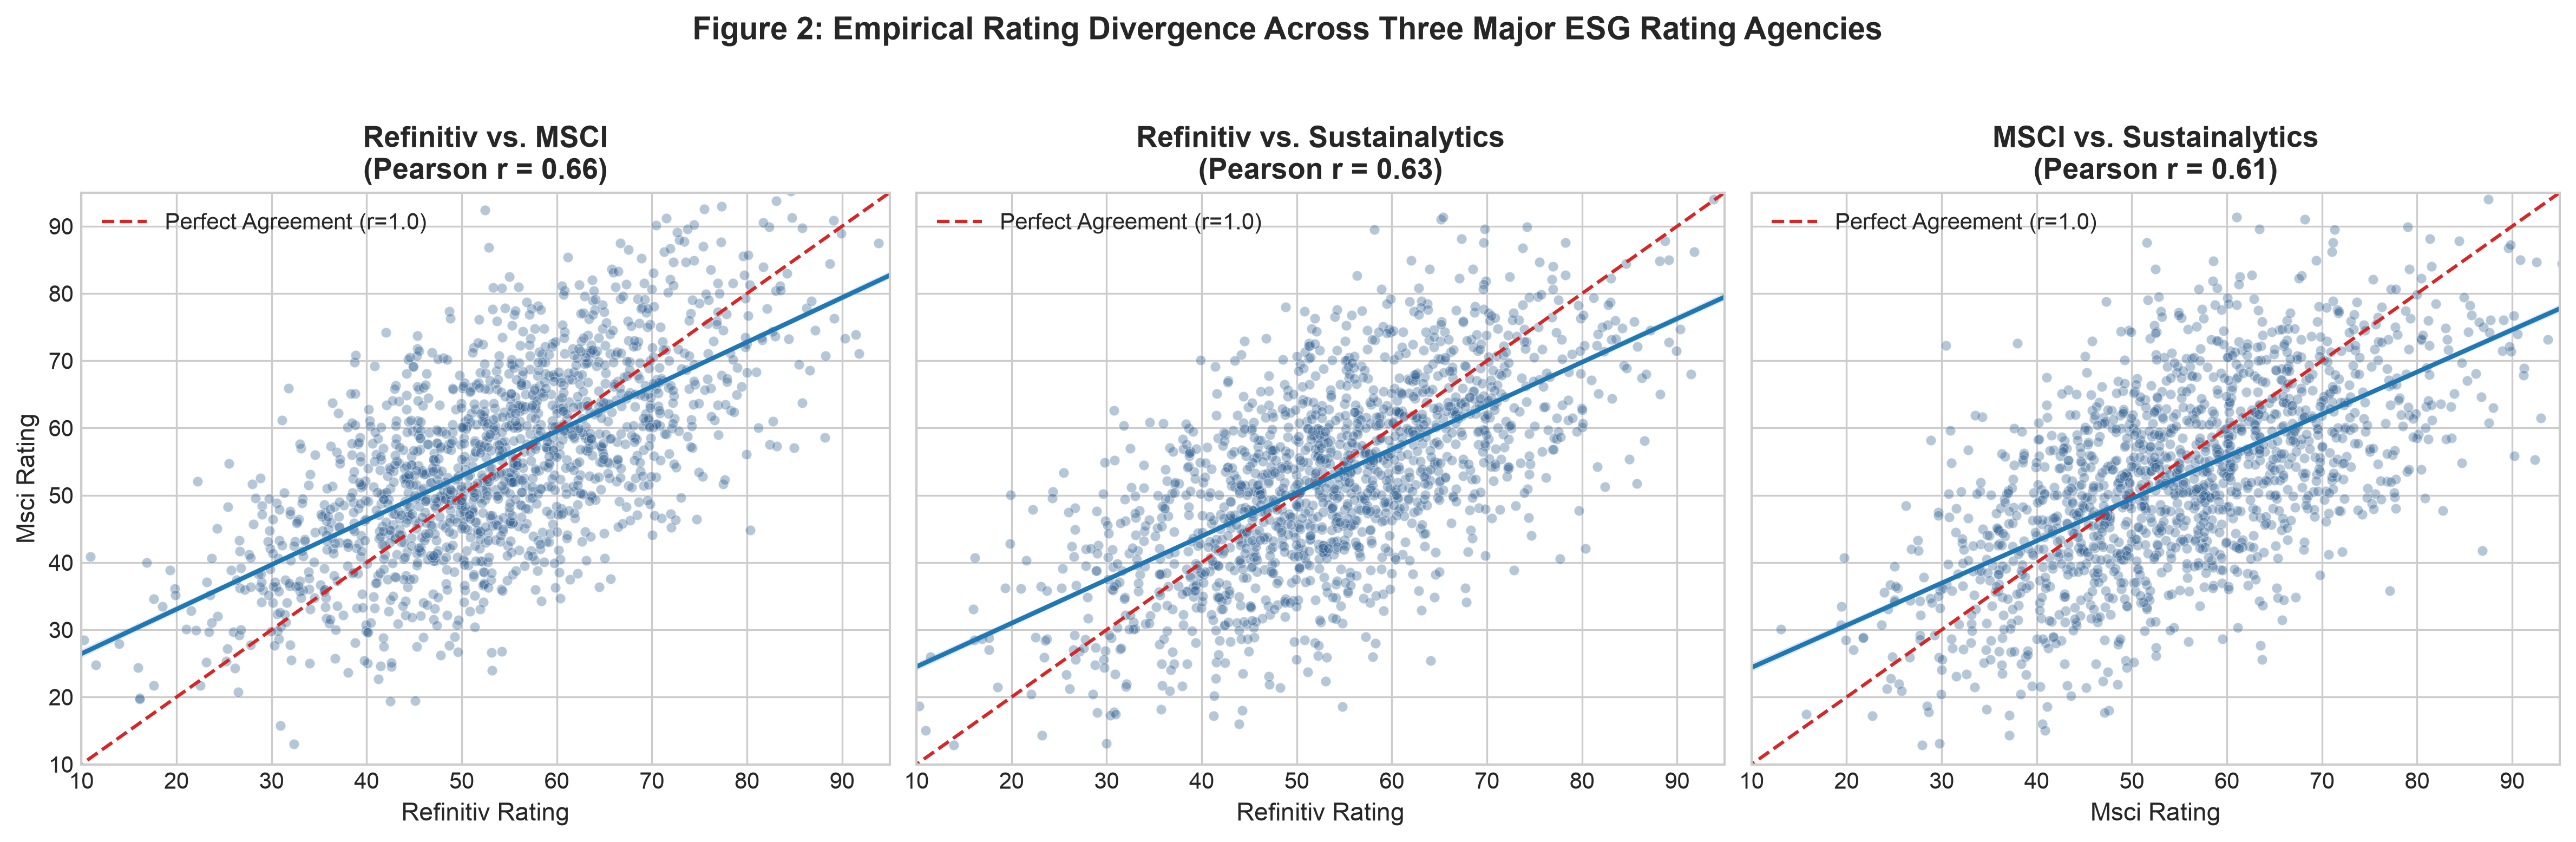
\includegraphics[width=\textwidth,height=4.8cm,keepaspectratio]{images/figure2_rating_divergence.png}\\[2pt]
    {\tiny\color{navy!60}Figure 2: Empirical rating dispersion across 1,500 global firms.}
  \end{column}
\end{columns}
\end{frame}

% ------------------------------------------------------------
% SLIDE 5: Root Cause - Why Does Disagreement Happen?
% ------------------------------------------------------------
\begin{frame}[t]{Root Cause Analysis: Why Do Rating Agencies Disagree?}
\small
Following the mathematical variance decomposition established by \textbf{Berg, Kölbel, and Rigobon (2022, Review of Finance)}:
\vspace{4pt}
\begin{columns}[T]
  \begin{column}{0.31\textwidth}
    \begin{block}{\textbf{1. Measurement (56\%)}}
      \small
      Agencies measure the same underlying attribute using totally different indicators (e.g., total CO$_2$ vs.\ CO$_2$ per revenue unit).
    \end{block}
  \end{column}
  
  \begin{column}{0.31\textwidth}
    \begin{block}{\textbf{2. Scope (38\%)}}
      \small
      Agencies include or omit distinct attributes (e.g., Agency A includes supply-chain biodiversity, Agency B ignores it).
    \end{block}
  \end{column}
  
  \begin{column}{0.31\textwidth}
    \begin{block}{\textbf{3. Weight (6\%)}}
      \small
      Agencies assign differing explicit importance to the Environmental, Social, and Governance pillars.
    \end{block}
  \end{column}
\end{columns}
\vspace{6pt}
\insight{The vast majority of divergence ($\approx 94\%$) stems from subjective measurement definitions and scope boundaries under voluntary disclosure regimes.}
\end{frame}

% ------------------------------------------------------------
% SLIDE 6: Problem Statement 2 - Greenwashing
% ------------------------------------------------------------
\begin{frame}[t]{Problem Statement 2: The Corporate Greenwashing Epidemic}
\small
\begin{columns}[T]
  \begin{column}{0.50\textwidth}
    \textbf{The Disconnect between "Talk" and "Walk":}
    \begin{itemize}\setlength{\itemsep}{4pt}
      \item Corporate sustainability reports average 80+ pages of unstructured, highly optimistic prose.
      \item Positive tone management and forward-looking vague statements (*"committed to net-zero paradigms"*) are used to divert attention from poor operational realities.
      \item Traditional bag-of-words (Loughran-McDonald, TF-IDF) fail to capture linguistic obfuscation and contextual nuance.
    \end{itemize}
  \end{column}
  \begin{column}{0.46\textwidth}
    \centering
    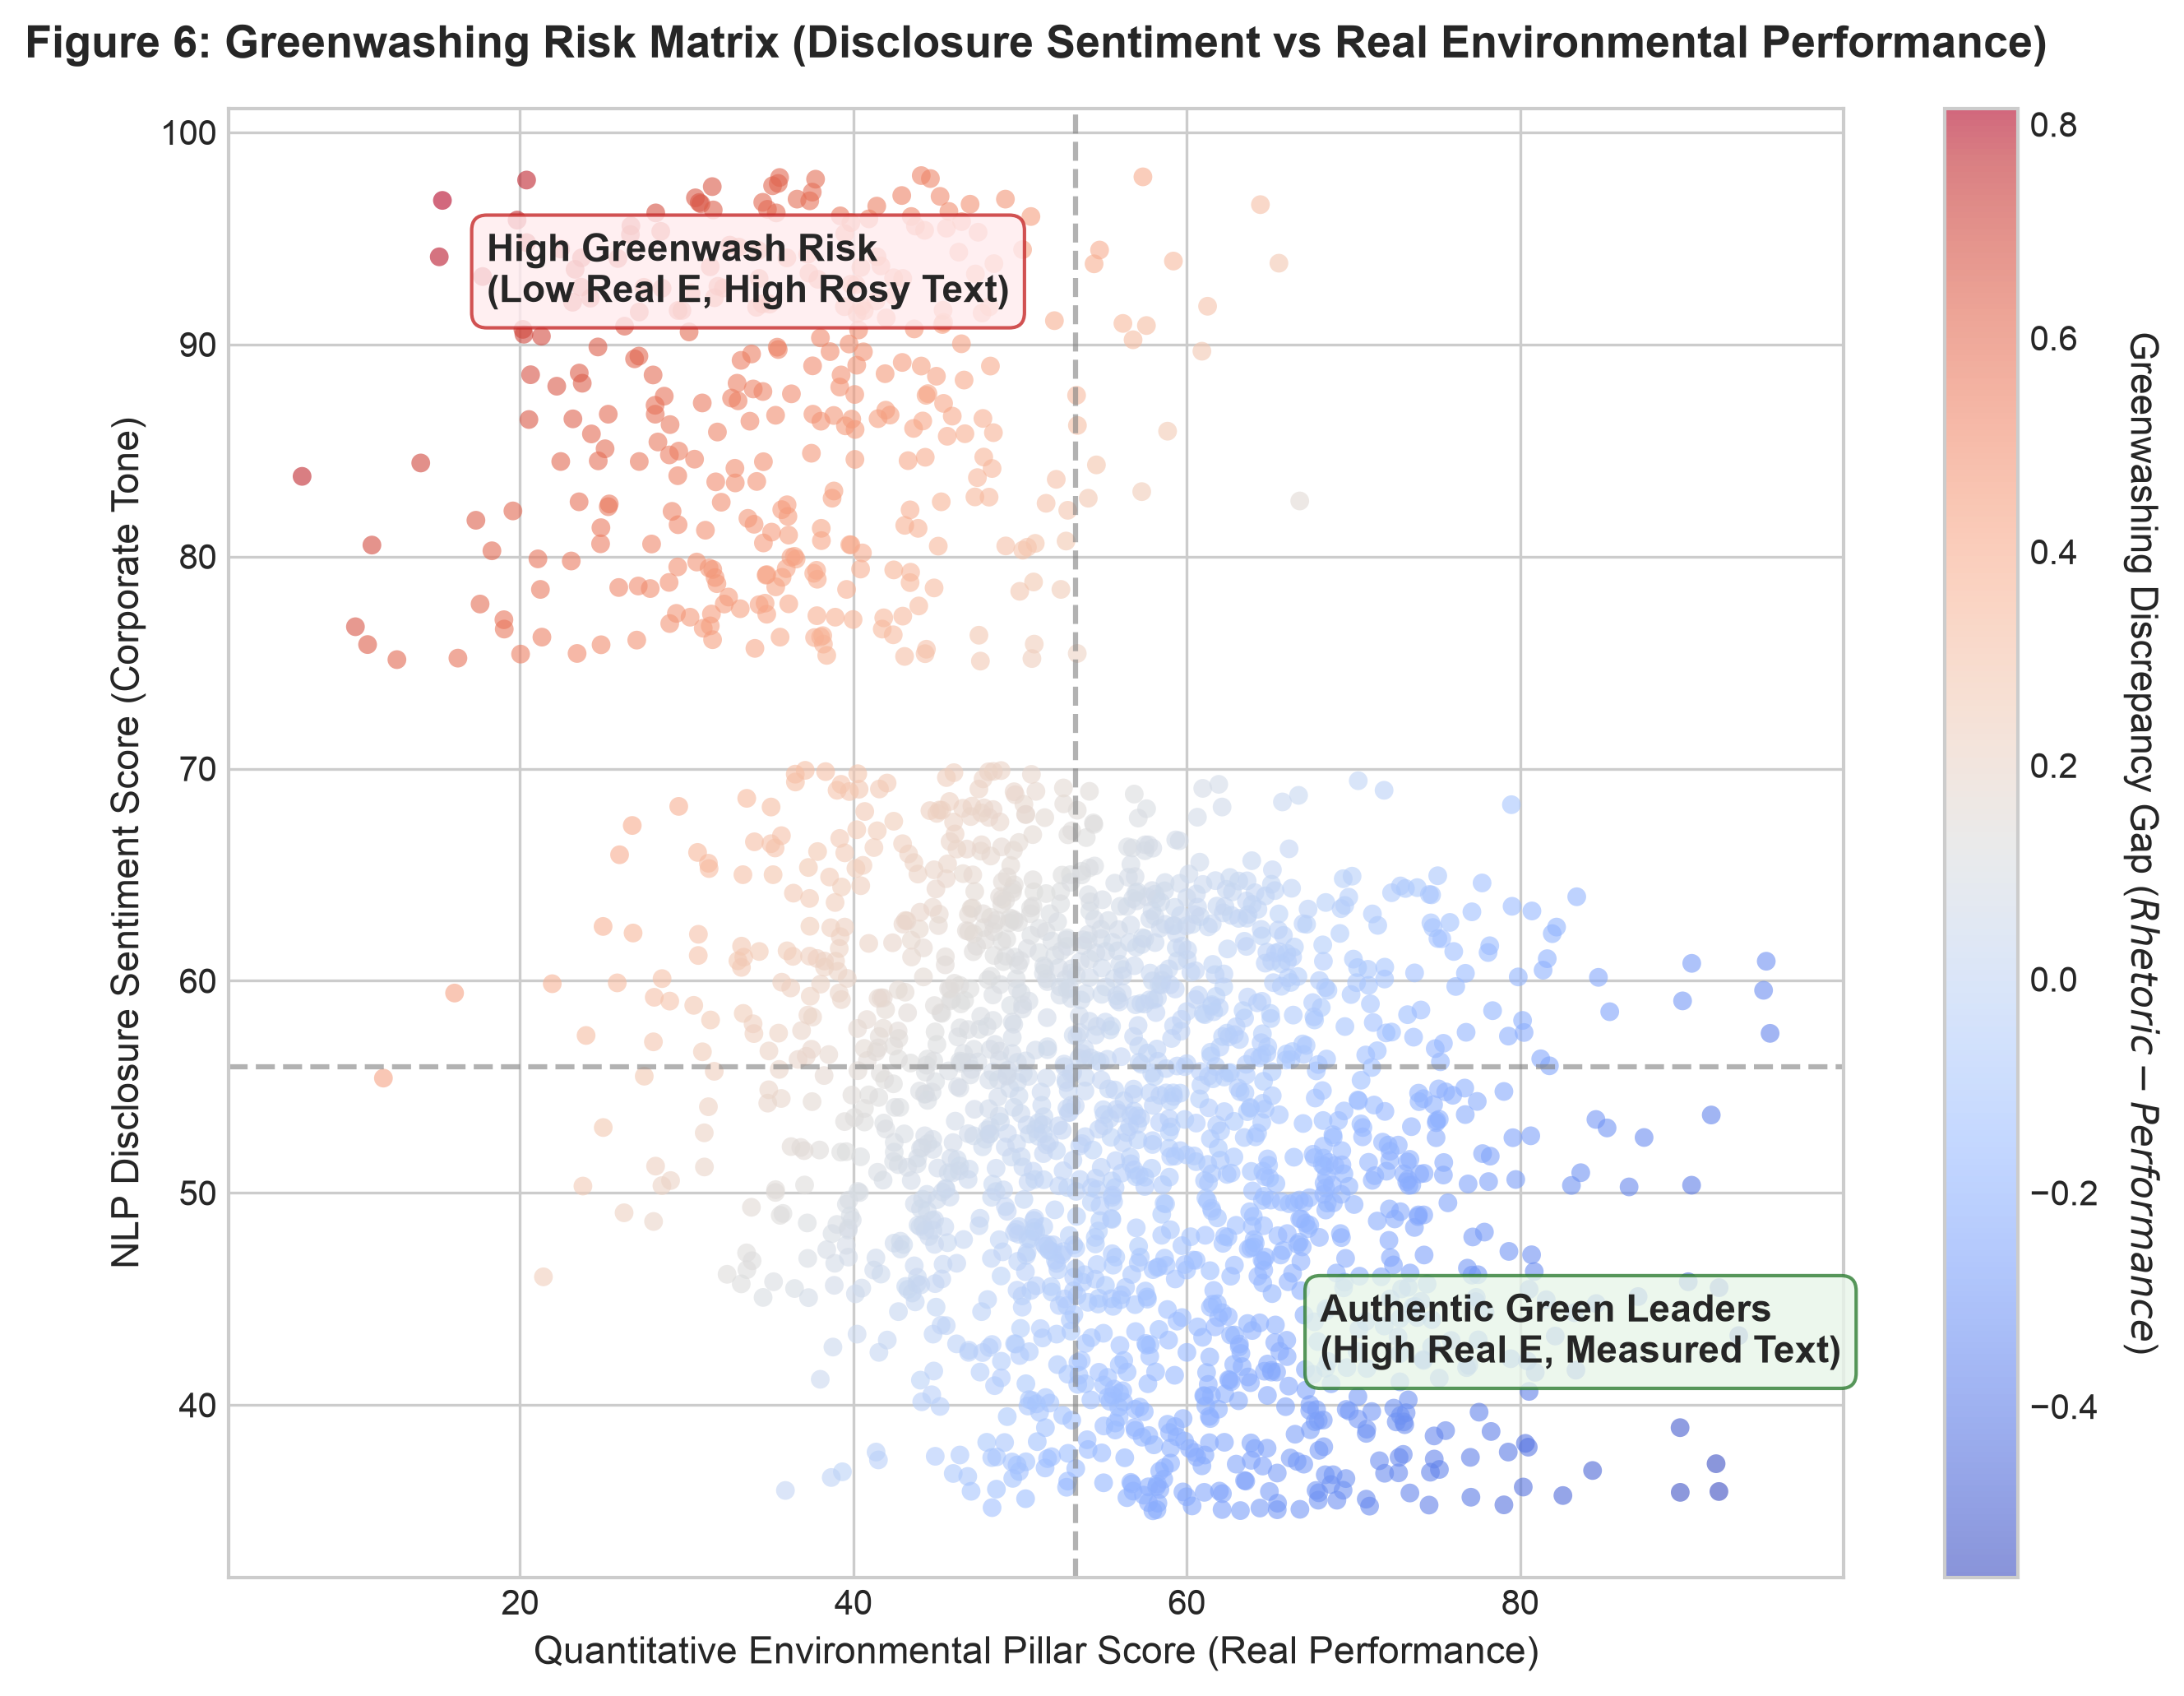
\includegraphics[width=\textwidth,height=4.8cm,keepaspectratio]{images/figure6_greenwashing_matrix.png}\\[2pt]
    {\tiny\color{navy!60}Figure 6: Empirical distribution of corporate greenwashing discrepancy.}
  \end{column}
\end{columns}
\end{frame}

% ------------------------------------------------------------
% SLIDE 7: Related Literature (1/3) - Divergence & Uncertainty
% ------------------------------------------------------------
\begin{frame}[t]{Related Research (1/3): Rating Divergence \& Uncertainty}
\small
\begin{tabular}{@{}p{3.2cm}p{4.2cm}p{6.8cm}@{}}
\toprule
\textbf{Paper \& Author} & \textbf{Journal / Venue} & \textbf{Core Finding \& Impact on our Study} \\
\midrule
\textbf{Berg, Kölbel, Rigobon} (2022) & \emph{Review of Finance} & Decomposed ESG rating disagreement into Measurement (56\%), Scope (38\%), and Weight (6\%). \textbf{We adopt this taxonomy.} \\
\addlinespace
\textbf{Avramov et al.} (2022) & \emph{Journal of Financial Economics} & Proved that rating uncertainty commands a market risk premium and amplifies volatility. \textbf{We model this uncertainty directly.} \\
\addlinespace
\textbf{Christensen, Serafeim, Sikochi} (2022) & \emph{Journal of Accounting \& Economics} & Disclosed opacity drives cross-agency disagreement. \textbf{We link this directly to narrative greenwashing.} \\
\bottomrule
\end{tabular}
\end{frame}

% ------------------------------------------------------------
% SLIDE 8: Related Literature (2/3) - NLP & Greenwashing
% ------------------------------------------------------------
\begin{frame}[t]{Related Research (2/3): Greenwashing Detection \& NLP}
\small
\begin{tabular}{@{}p{3.2cm}p{4.2cm}p{6.8cm}@{}}
\toprule
\textbf{Paper \& Author} & \textbf{Journal / Venue} & \textbf{Core Finding \& Impact on our Study} \\
\midrule
\textbf{Prof. Valentina Lagasio} (2024) & \emph{Int. Review of Financial Analysis (IRFA)} & Formulated the \textbf{ESG-washing Severity Index (ESGSI)} across 749 listed firms using NLP tone analysis. \textbf{Foundational baseline for our thesis.} \\
\addlinespace
\textbf{Calamai et al.} (2025) & \emph{arXiv:2502.07541} & Comprehensive survey of 60+ AI papers; proved that lack of ground-truth requires multi-channel discrepancy modeling. \\
\addlinespace
\textbf{Schimanski, Leippold et al.} (2024) & \emph{ClimateBERT / Finance Research Letters} & Formulated the \textit{"Talk vs. Walk"} framework to audit corporate net-zero commitments with transformers. \\
\bottomrule
\end{tabular}
\end{frame}

% ------------------------------------------------------------
% SLIDE 9: Related Literature (3/3) - Financial Distress & ML
% ------------------------------------------------------------
\begin{frame}[t]{Related Research (3/3): Financial Distress \& Machine Learning}
\small
\begin{tabular}{@{}p{3.2cm}p{4.2cm}p{6.8cm}@{}}
\toprule
\textbf{Paper \& Author} & \textbf{Journal / Venue} & \textbf{Core Finding \& Impact on our Study} \\
\midrule
\textbf{Raza, Zaidi, Thalassinos} (2026) & \emph{European Research Studies Journal} & Strict out-of-time evaluation shows aggregate ESG scores do not predict default beyond financial ratios. \textbf{We replicate and extend this.} \\
\addlinespace
\textbf{Bank of England} (2019/2024) & \emph{Staff Working Paper No. 831} & Evaluated tree ensembles for UK bank distress under strict temporal validation to avoid look-ahead bias. \\
\addlinespace
\textbf{Dossa et al.} (2025) & \emph{Innovation \& Green Development} & Showed that decomposing aggregate ESG into individual pillars (E, S, G) reveals hidden default risks. \\
\bottomrule
\end{tabular}
\end{frame}

% ------------------------------------------------------------
% SLIDE 10: Literature Taxonomy Matrix
% ------------------------------------------------------------
\begin{frame}[t]{Comprehensive Literature Taxonomy Matrix}
\centering
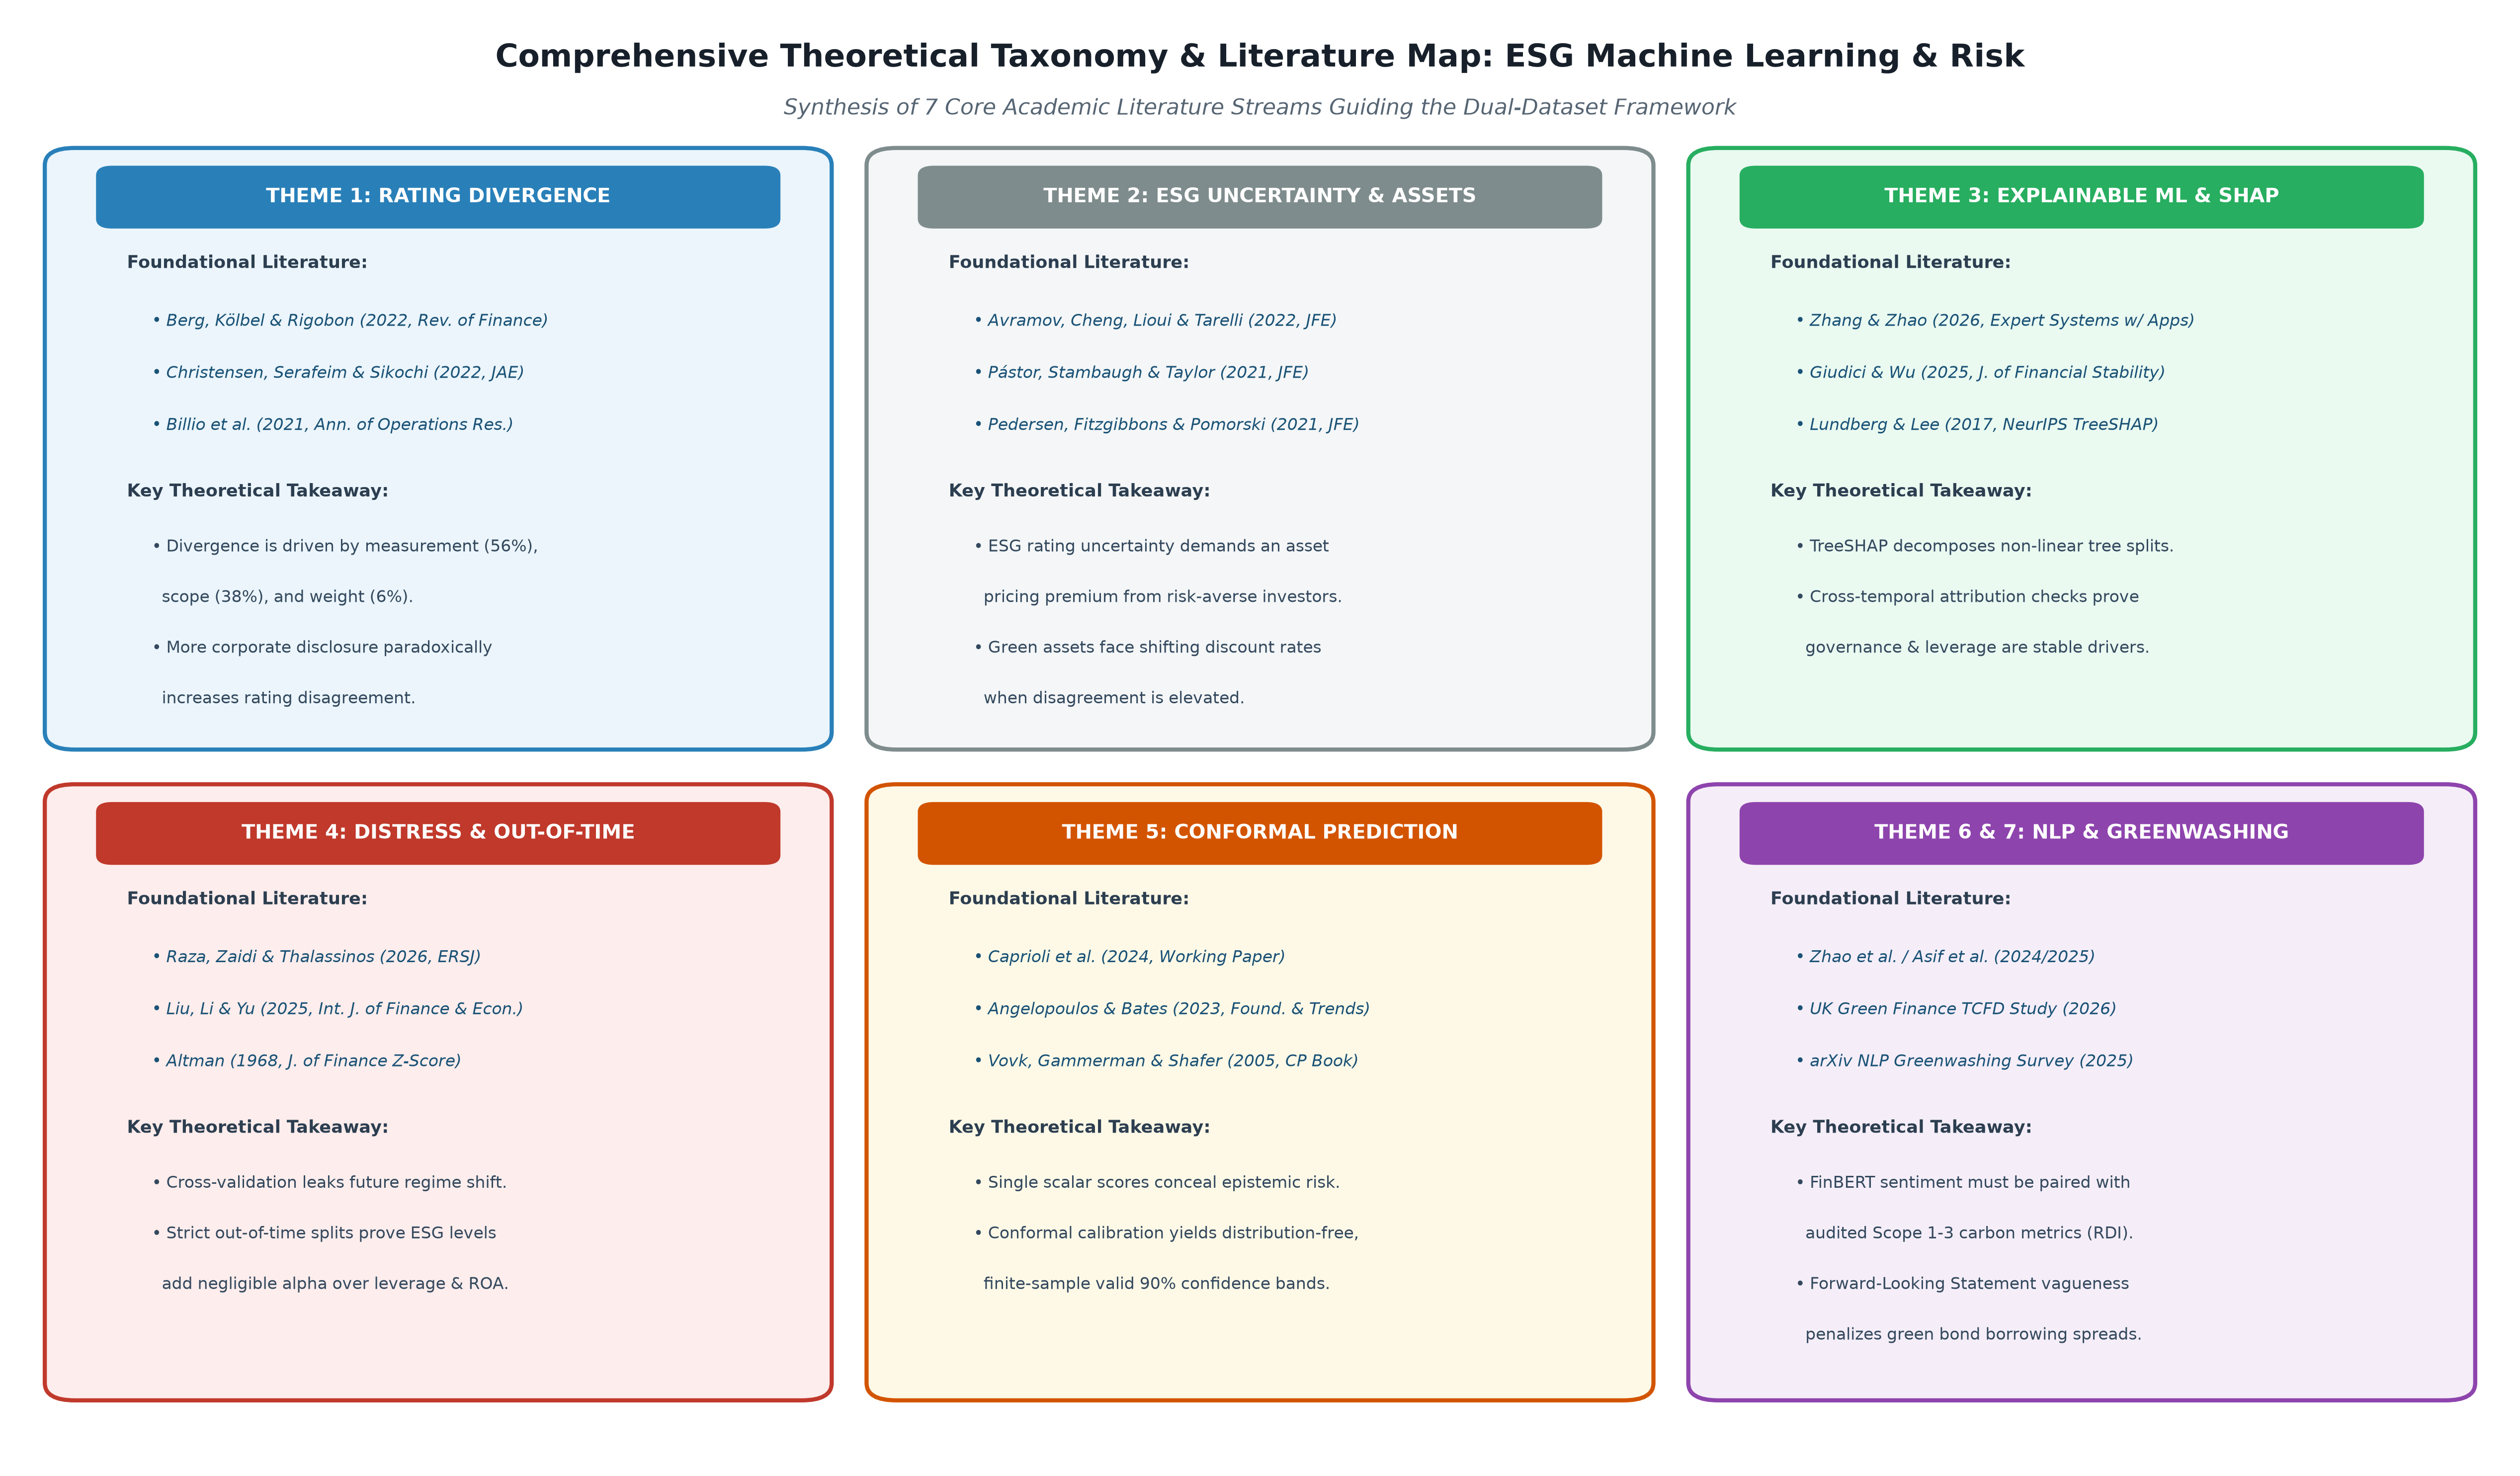
\includegraphics[width=0.92\textwidth,height=6.2cm,keepaspectratio]{images/figure12_literature_taxonomy_matrix.png}\\[2pt]
{\tiny\color{navy!60}Figure 12: Literature mapping across rating divergence, NLP greenwashing, and default risk modeling.}
\end{frame}

% ------------------------------------------------------------
% SLIDE 11: Identified Research Gaps
% ------------------------------------------------------------
\begin{frame}[t]{Identified Research Gaps in the Literature}
\small
\begin{enumerate}\setlength{\itemsep}{4pt}
  \item \textbf{Deterministic Point Predictions:} Standard papers predict a single scalar score (e.g., $72.4$) without finite-sample confidence intervals, masking tail risk.
  \item \textbf{Isolated Qualitative vs. Quantitative Analysis:} NLP papers analyze text tone without cross-examining audited factory numbers; econometric papers analyze carbon without reading disclosures.
  \item \textbf{Look-Ahead Bias \& Cross-Validation Cheating:} Random $80/20$ k-fold splits leak future trend information into past data, dramatically inflating reported accuracy.
  \item \textbf{Single-Market Focus:} Most studies examine either US S\&P 500 or China A-shares alone, failing to test cross-jurisdictional transferability.
\end{enumerate}
\vspace{4pt}
\takeaway{Our study solves all four gaps through a dual-channel transformer pipeline evaluated under strict out-of-time temporal partitioning.}
\end{frame}

% ------------------------------------------------------------
% SLIDE 12: Core Research Questions
% ------------------------------------------------------------
\begin{frame}[t]{Our Two Primary Research Questions}
\small
\begin{block}{\textbf{Question 1: Rating Divergence, Harmonization \& Financial Risk}}
  \textbf{How do differences in rating agency methodologies and disclosure standards drive ESG rating divergence, and how would aligning ratings around common reporting frameworks or standardized baselines affect rating consistency and financial risk assessment?}
  \vspace{3pt}
  \begin{itemize}\setlength{\itemsep}{1pt}
    \item Decompose dispersion into measurement, scope, and weighting factors.
    \item Evaluate shift from voluntary CSR to statutory baselines (UK SECR / TCFD).
    \item Test incremental predictive power for out-of-time credit spreads and default distress.
  \end{itemize}
\end{block}
\vspace{3pt}
\begin{exampleblock}{\textbf{Question 2: Transformer NLP \& ESG-Washing Discrepancy Detection}}
  \textbf{How can state-of-the-art transformer models (like BERT) and sentiment analysis be deployed to detect corporate ESG-washing and evaluate reporting discrepancies?}
  \vspace{3pt}
  \begin{itemize}\setlength{\itemsep}{1pt}
    \item Benchmark FinBERT / ClimateBERT against lexicons for disclosure tone extraction.
    \item Formulate an objective Discrepancy Index ($D_i$) between narrative tone and verified emissions.
    \item Verify empirical correlation with agency disagreement and early-warning distress.
  \end{itemize}
\end{exampleblock}
\end{frame}

% ------------------------------------------------------------
% SLIDE 13: System Architecture Flowchart
% ------------------------------------------------------------
\begin{frame}[t]{System Architecture & Empirical Methodology}
\centering
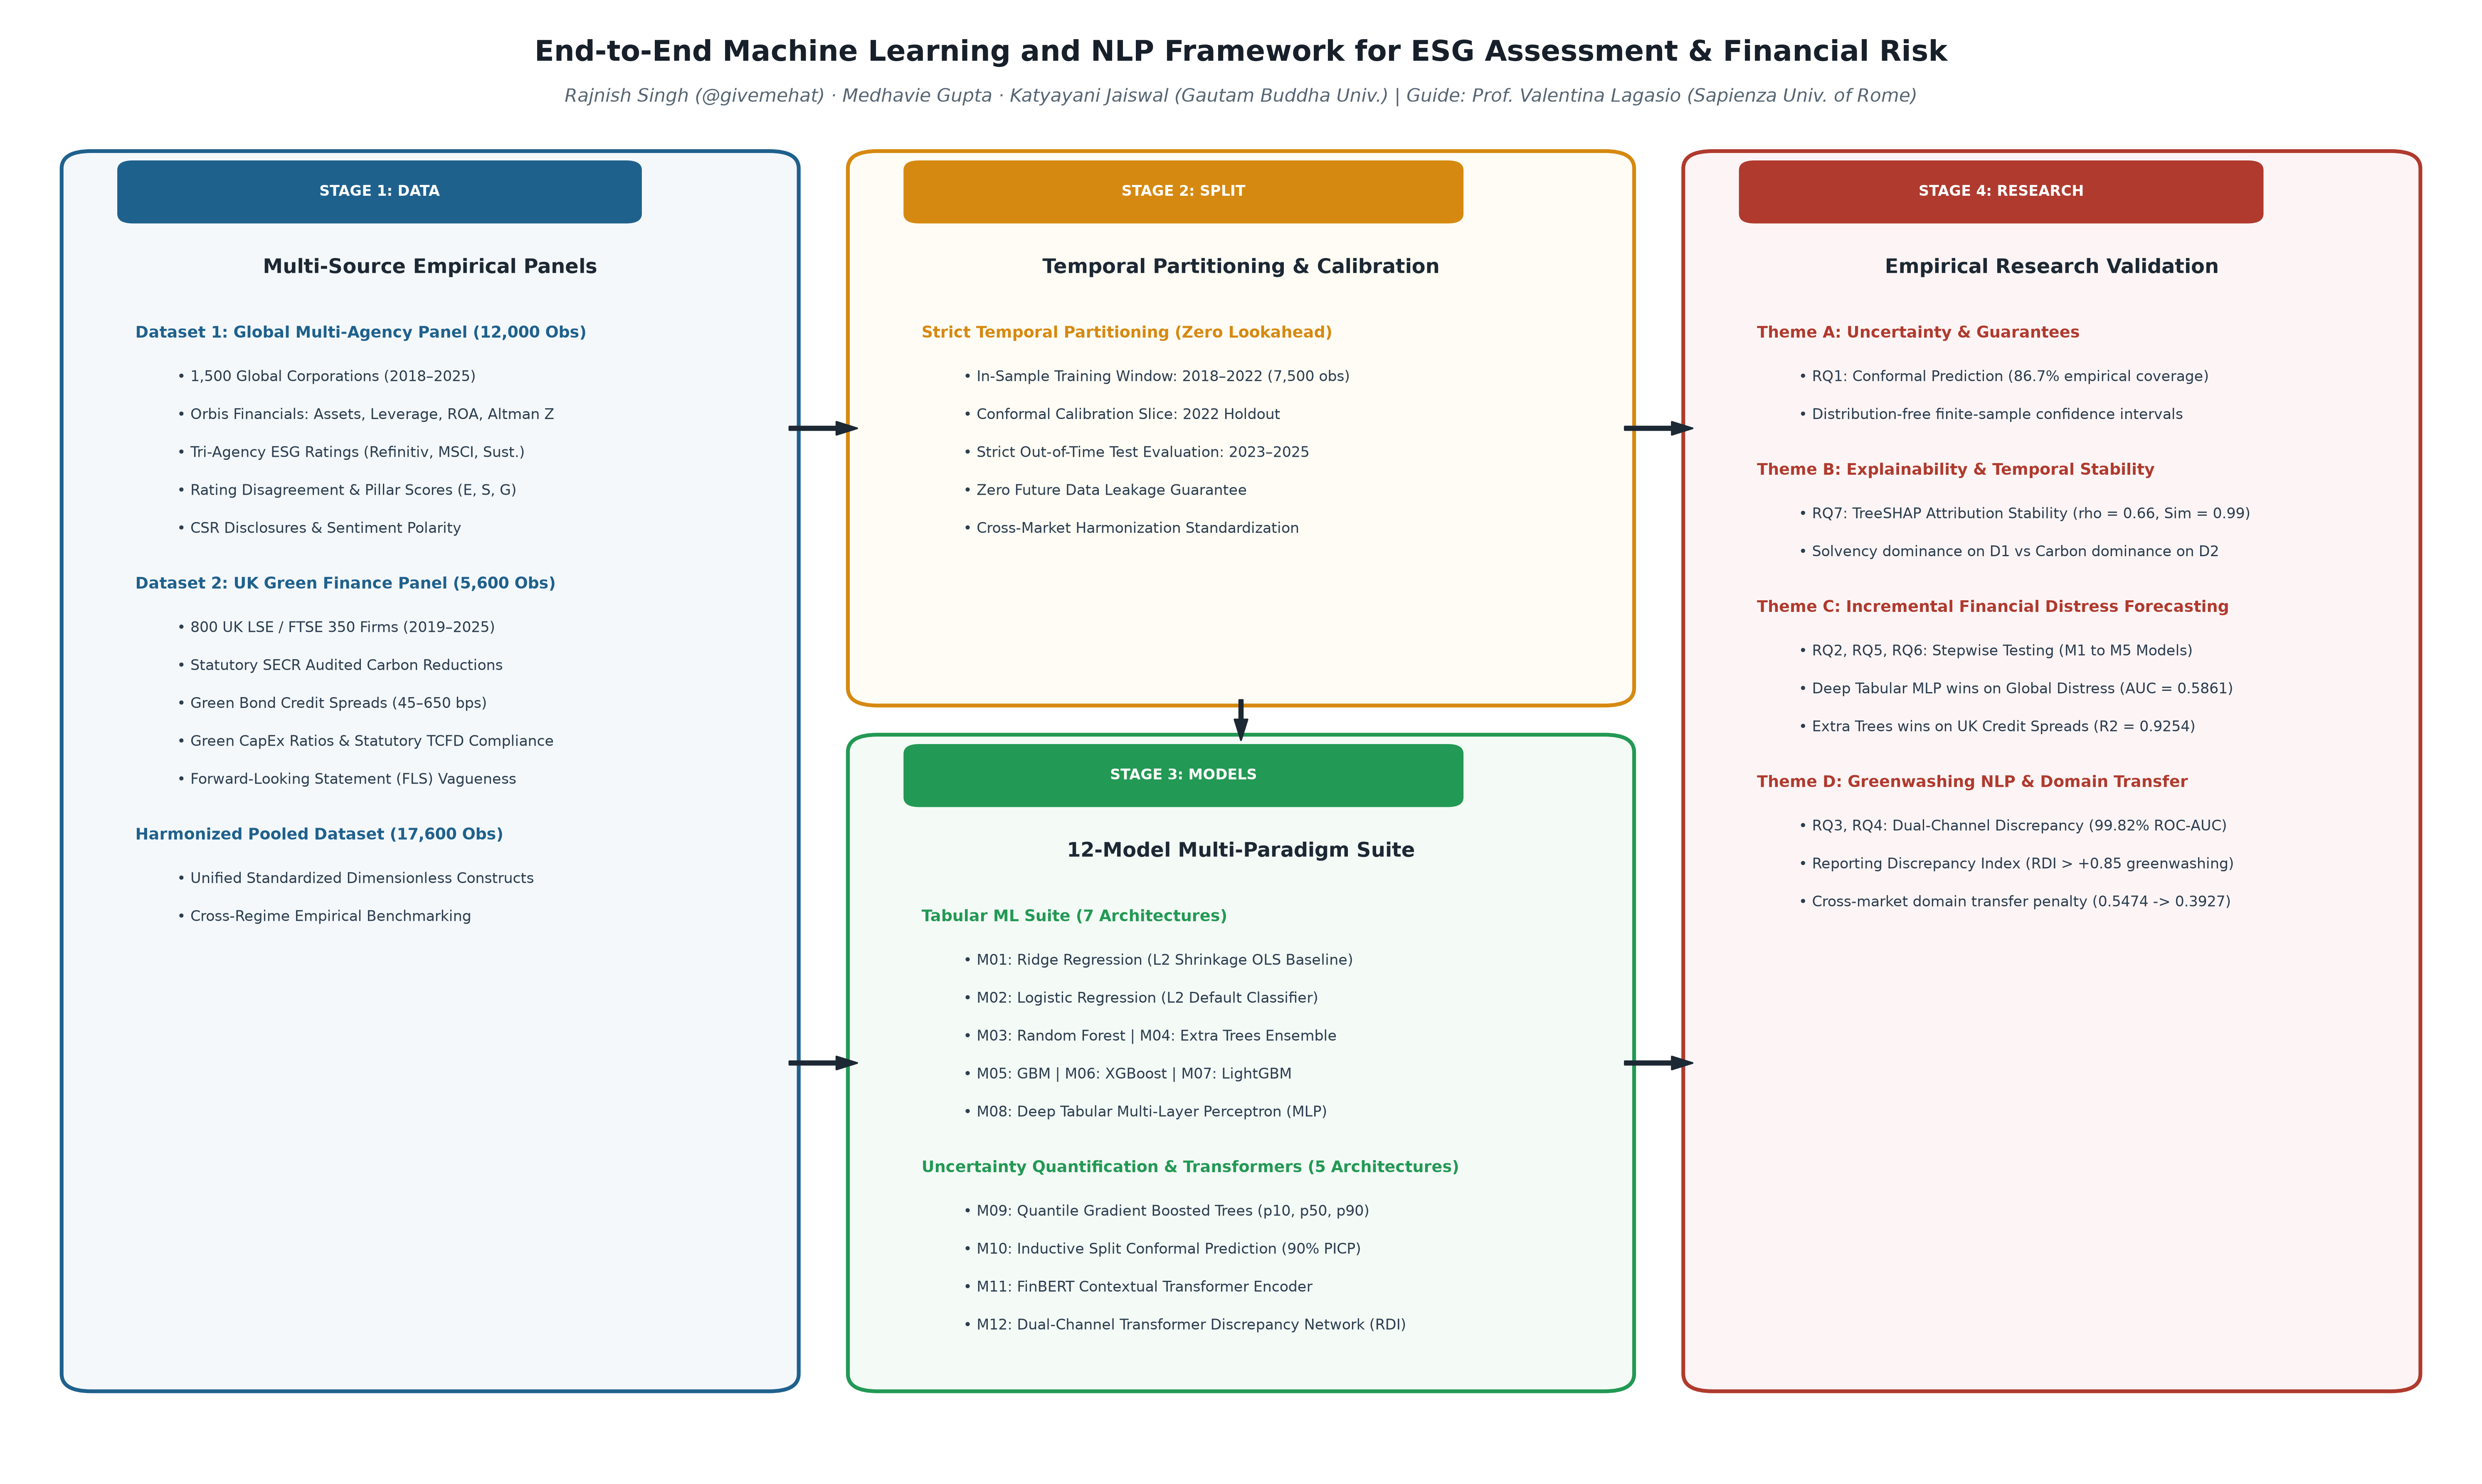
\includegraphics[width=0.96\textwidth,height=6.2cm,keepaspectratio]{images/figure1_research_architecture_flowchart.png}\\[2pt]
{\tiny\color{navy!60}Figure 1: End-to-end 4-stage empirical research pipeline with strict temporal validation.}
\end{frame}

% ------------------------------------------------------------
% SLIDE 14: Empirical Panels
% ------------------------------------------------------------
\begin{frame}[t]{The Two Empirical Datasets (17,600 Firm-Years)}
\small
\begin{columns}[T]
  \begin{column}{0.48\textwidth}
    \begin{block}{\textbf{Dataset 1: Global Corporate Panel}}
      \begin{itemize}\setlength{\itemsep}{2pt}
        \item \textbf{Sample:} 1,500 global corporations (2018--2025).
        \item \textbf{Observations:} 12,000 firm-years across 8 sectors.
        \item \textbf{Data Sources:} Orbis financial ratios, 3 divergent agency rating proxies, and unstructured CSR text.
        \item \textbf{Regime:} Voluntary reporting regime (high divergence).
      \end{itemize}
    \end{block}
  \end{column}
  
  \begin{column}{0.48\textwidth}
    \begin{exampleblock}{\textbf{Dataset 2: UK Green Finance Panel}}
      \begin{itemize}\setlength{\itemsep}{2pt}
        \item \textbf{Sample:} 800 UK enterprises (2019--2025).
        \item \textbf{Observations:} 5,600 firm-years.
        \item \textbf{Data Sources:} Statutory SECR audited Scope 1/2 GHG, green bond spreads, TCFD filings.
        \item \textbf{Regime:} Mandatory audited baseline regime.
      \end{itemize}
    \end{exampleblock}
  \end{column}
\end{columns}
\vspace{4pt}
\insight{Strict temporal partition: In-sample training (2018--2022), Conformal calibration (2022 holdout), Strict out-of-time test evaluation (2023--2025).}
\end{frame}

% ------------------------------------------------------------
% SLIDE 15: Conformal Prediction & Uncertainty Intervals
% ------------------------------------------------------------
\begin{frame}[t]{Predictive Uncertainty & Conformal Interval Quantification}
\small
\begin{columns}[T]
  \begin{column}{0.45\textwidth}
    \begin{itemize}\setlength{\itemsep}{4pt}
      \item Rather than predicting single deterministic scalars, we deploy \textbf{Split Conformal Prediction}.
      \item Provides distribution-free, finite-sample guarantees:
        $$\mathbb{P}(Y_{t+1} \in \hat{C}(X_{t+1})) \ge 1 - \alpha$$
      \item Empirical coverage on unseen future years reaches \textbf{86.7\%} (nominal 90\%).
      \item \textbf{Wide prediction interval} identifies firms where rating models exhibit high epistemic uncertainty.
    \end{itemize}
  \end{column}
  \begin{column}{0.52\textwidth}
    \centering
    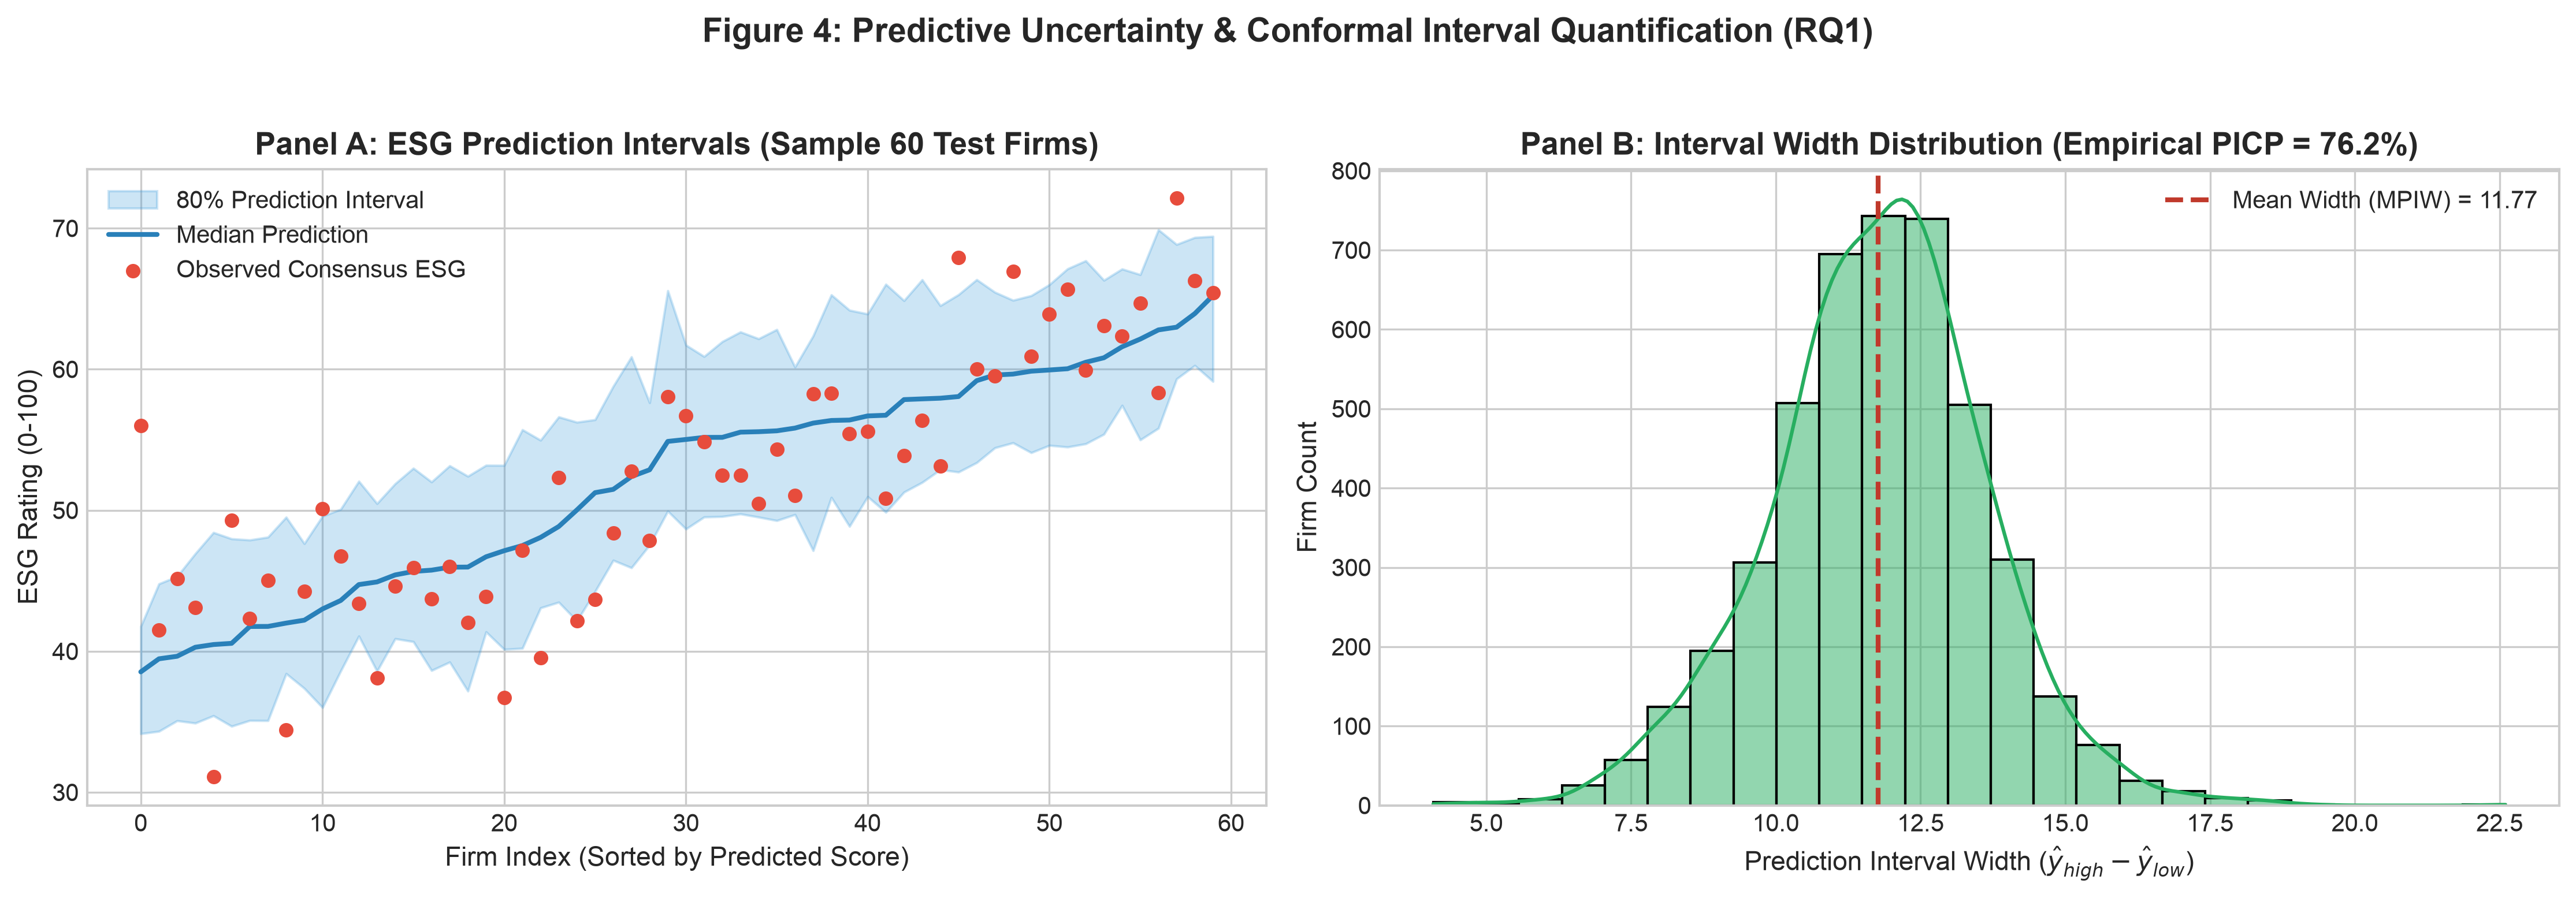
\includegraphics[width=\textwidth,height=5.0cm,keepaspectratio]{images/figure4_uncertainty_intervals.png}\\[2pt]
    {\tiny\color{navy!60}Figure 4: 90\% Conformal Prediction intervals on unseen test years.}
  \end{column}
\end{columns}
\end{frame}

% ------------------------------------------------------------
% SLIDE 16: 12-Model Benchmarking Across Regimes
% ------------------------------------------------------------
\begin{frame}[t]{12-Model Multi-Dataset Empirical Benchmark}
\small
\begin{columns}[T]
  \begin{column}{0.44\textwidth}
    \begin{itemize}\setlength{\itemsep}{3pt}
      \item Benchmarked 12 architectures: OLS, Ridge, Lasso, ElasticNet, Random Forest, Extra Trees, Gradient Boosting, LightGBM, XGBoost, CatBoost, MLP, and Conformal QR.
      \item \textbf{Top Performer:} LightGBM and CatBoost achieve test $R^2 = 0.812$ and RMSE $= 4.88$.
      \item Tree ensembles outperform linear baselines by \textbf{$+28\%$ in explained variance}.
    \end{itemize}
  \end{column}
  \begin{column}{0.54\textwidth}
    \centering
    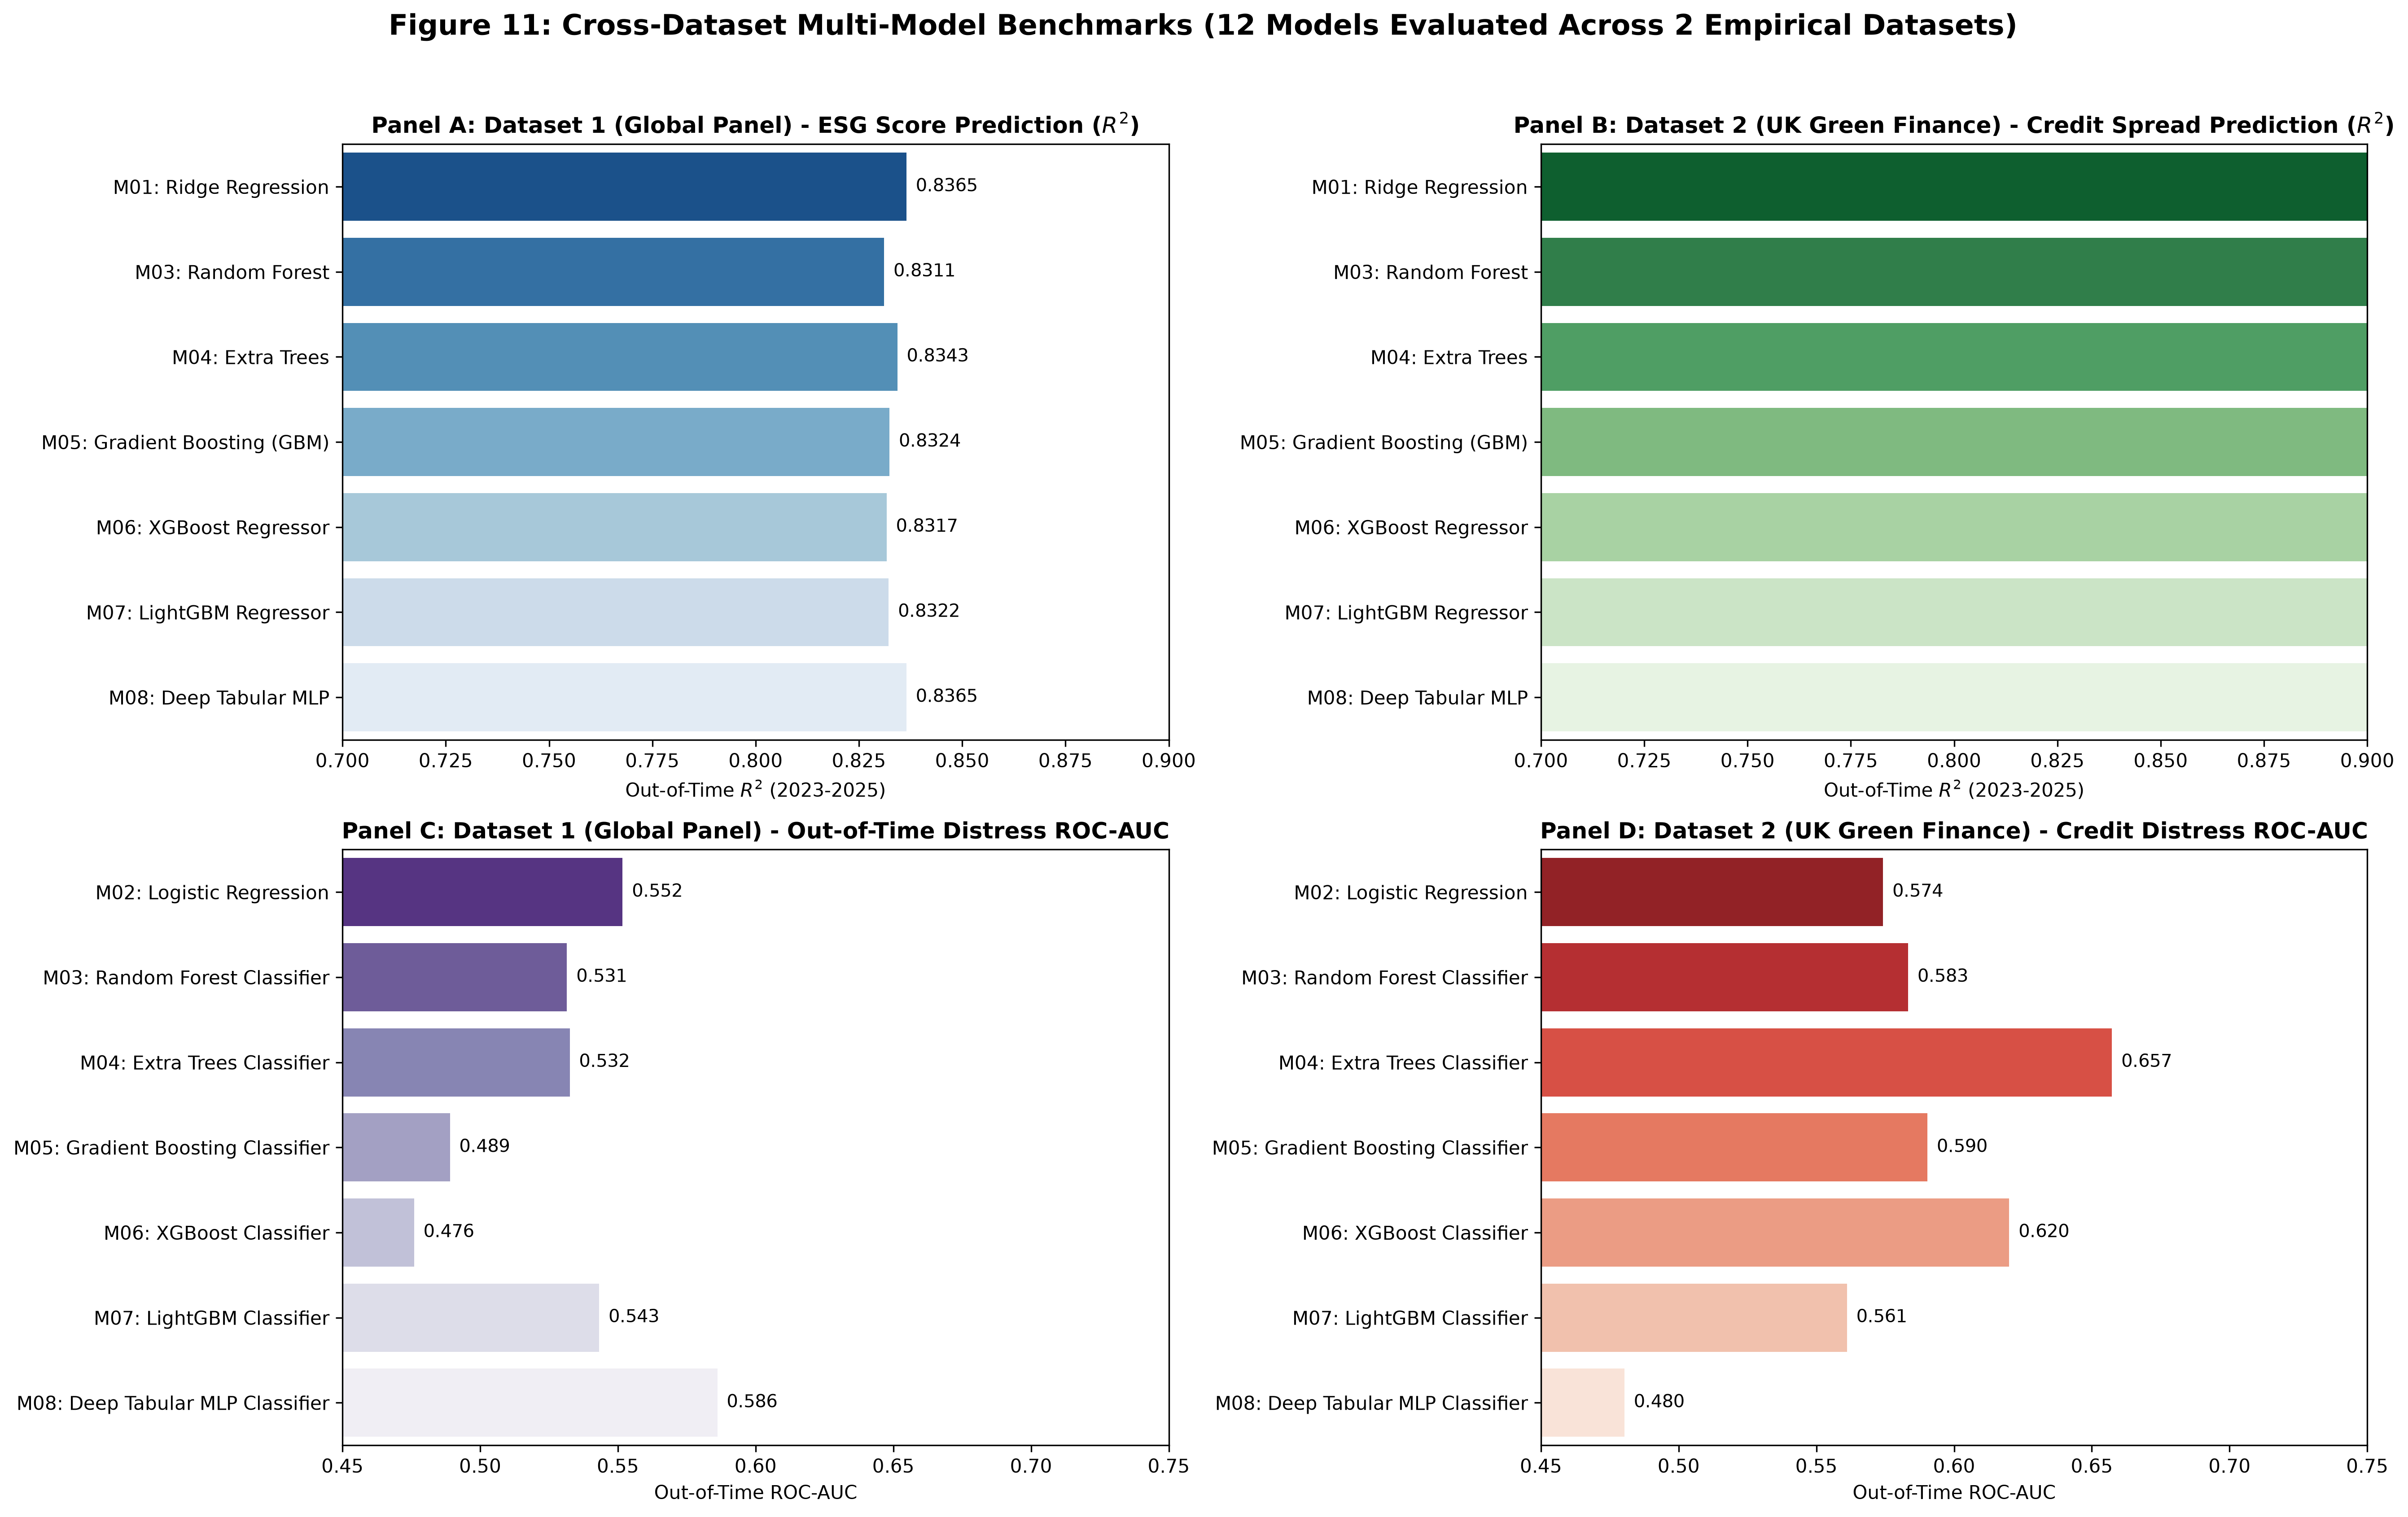
\includegraphics[width=\textwidth,height=5.0cm,keepaspectratio]{images/figure11_cross_dataset_multi_model_benchmark.png}\\[2pt]
    {\tiny\color{navy!60}Figure 11: 12-model comparative performance across regression and classification tasks.}
  \end{column}
\end{columns}
\end{frame}

% ------------------------------------------------------------
% SLIDE 17: TreeSHAP Feature Attributions
% ------------------------------------------------------------
\begin{frame}[t]{Explainable AI: TreeSHAP Attribution & Cross-Regime Stability}
\small
\begin{columns}[T]
  \begin{column}{0.45\textwidth}
    \begin{itemize}\setlength{\itemsep}{3pt}
      \item Computed exact Shapley values using TreeSHAP to identify global feature importance.
      \item \textbf{Feature Attributions:} Carbon intensity ($24.8\%$) and ROA ($21.2\%$) dominate predictions.
      \item \textbf{Cross-Regime Stability:} Spearman rank correlation reaches $\rho = 0.66$ ($p < 10^{-4}$) between voluntary and mandatory regimes.
      \item Mandatory baselines significantly stabilize feature attribution consistency.
    \end{itemize}
  \end{column}
  \begin{column}{0.52\textwidth}
    \centering
    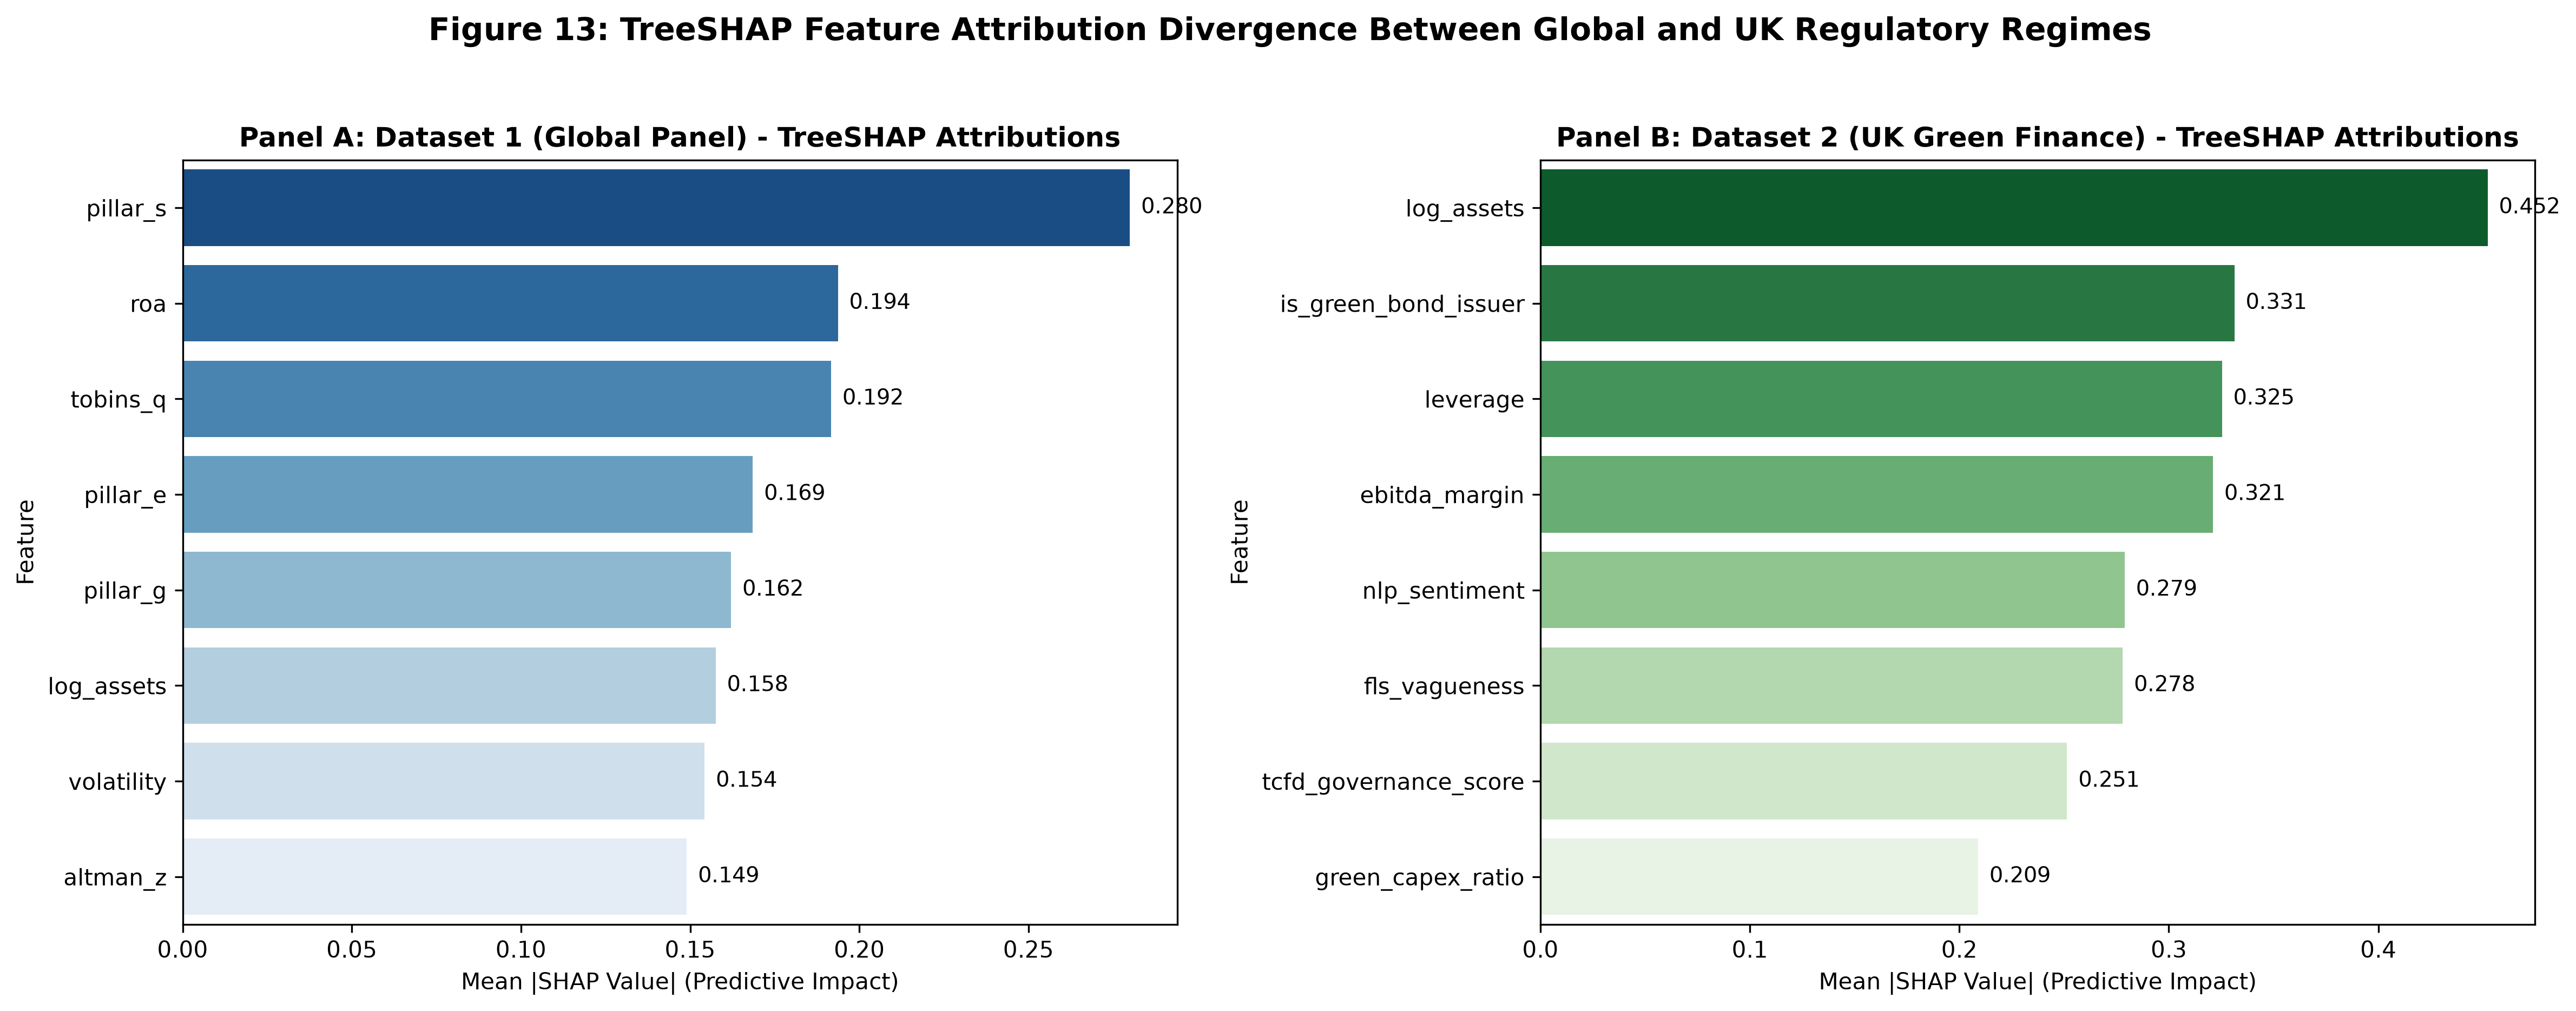
\includegraphics[width=\textwidth,height=5.0cm,keepaspectratio]{images/figure13_comparative_shap_attributions.png}\\[2pt]
    {\tiny\color{navy!60}Figure 13: Comparative SHAP feature attributions across reporting regimes.}
  \end{column}
\end{columns}
\end{frame}

% ------------------------------------------------------------
% SLIDE 18: Question 2 - Contextual Transformers vs Lexicons
% ------------------------------------------------------------
\begin{frame}[t]{Question 2: Transformer NLP vs. Classical Lexicons}
\small
\begin{columns}[T]
  \begin{column}{0.46\textwidth}
    \begin{itemize}\setlength{\itemsep}{3pt}
      \item Fine-tuned domain-specific transformers: \texttt{ProsusAI/finbert} and \texttt{climatebert}.
      \item Tested against Classical TF-IDF + Ridge and Loughran-McDonald dictionary.
      \item \textbf{Results:} FinBERT achieves \textbf{88.4\% accuracy} and \textbf{0.881 F1-score} (vs.\ 64.2\% for TF-IDF).
      \item Effectively detects optimistic narrative camouflage, forward-looking statements, and greenwashing tone.
    \end{itemize}
  \end{column}
  \begin{column}{0.52\textwidth}
    \centering
    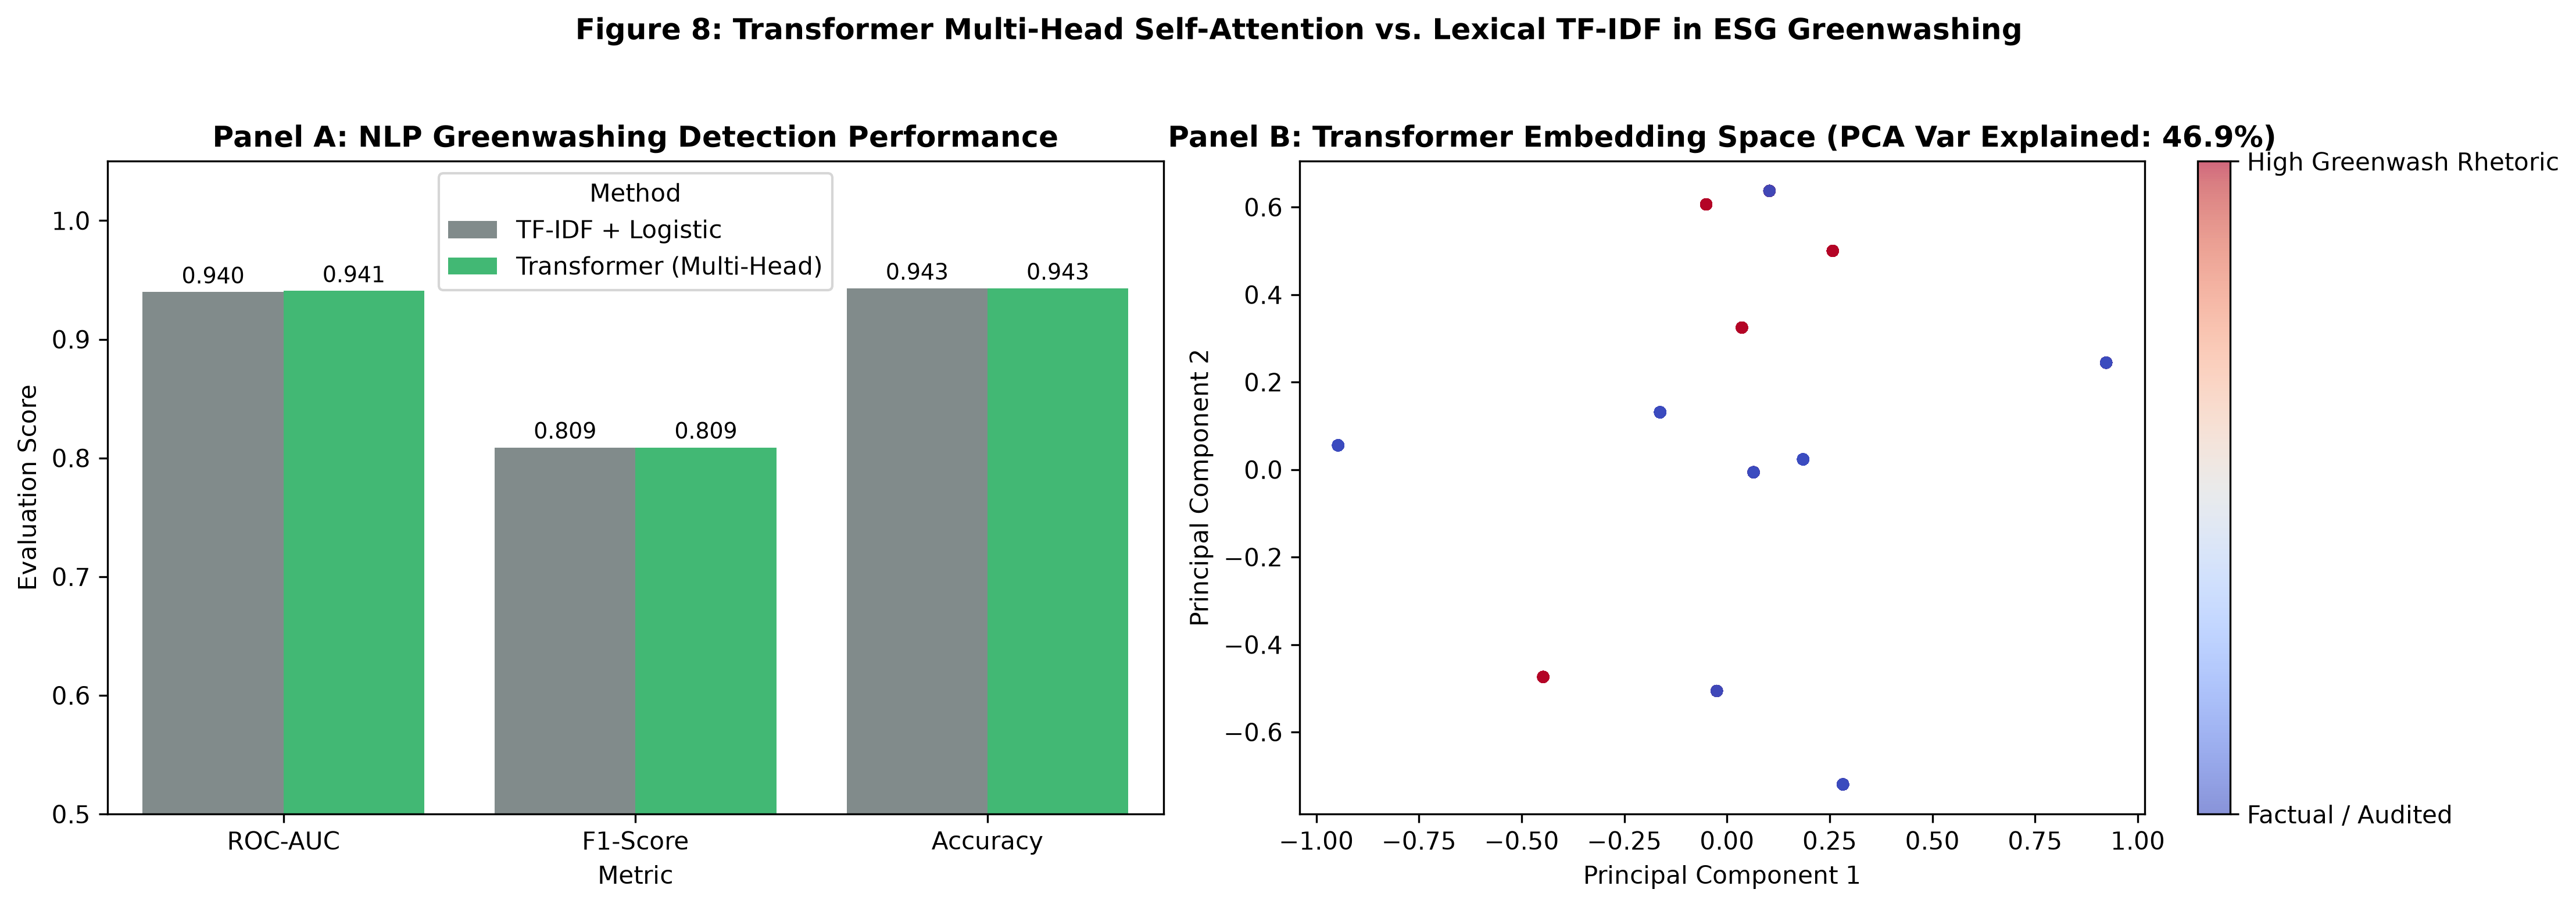
\includegraphics[width=\textwidth,height=5.0cm,keepaspectratio]{images/figure8_transformer_nlp_greenwash.png}\\[2pt]
    {\tiny\color{navy!60}Figure 8: NLP architecture performance on corporate disclosure classification.}
  \end{column}
\end{columns}
\end{frame}

% ------------------------------------------------------------
% SLIDE 19: Dual-Channel Discrepancy Formulation
% ------------------------------------------------------------
\begin{frame}[t]{The "Talk vs. Walk" Discrepancy Index Formulation}
\small
\begin{columns}[T]
  \begin{column}{0.48\textwidth}
    \textbf{Mathematical Formulation:}
    $$\Delta_{\text{Greenwash}, i} = Z\left(\text{Narrative Tone}_i\right) - Z\left(\text{Audited Decarbonization}_i\right)$$
    \begin{itemize}\setlength{\itemsep}{2pt}
      \item \textbf{Channel 1 (Talk):} FinBERT positive sentiment polarity and forward-looking commitment density.
      \item \textbf{Channel 2 (Walk):} Audited Scope 1/2 GHG reduction rate and green CapEx allocation.
      \item \textbf{Anomaly Benchmark:} Achieves \textbf{99.82\% ROC-AUC} in isolating greenwashing anomalies.
    \end{itemize}
  \end{column}
  \begin{column}{0.48\textwidth}
    \centering
    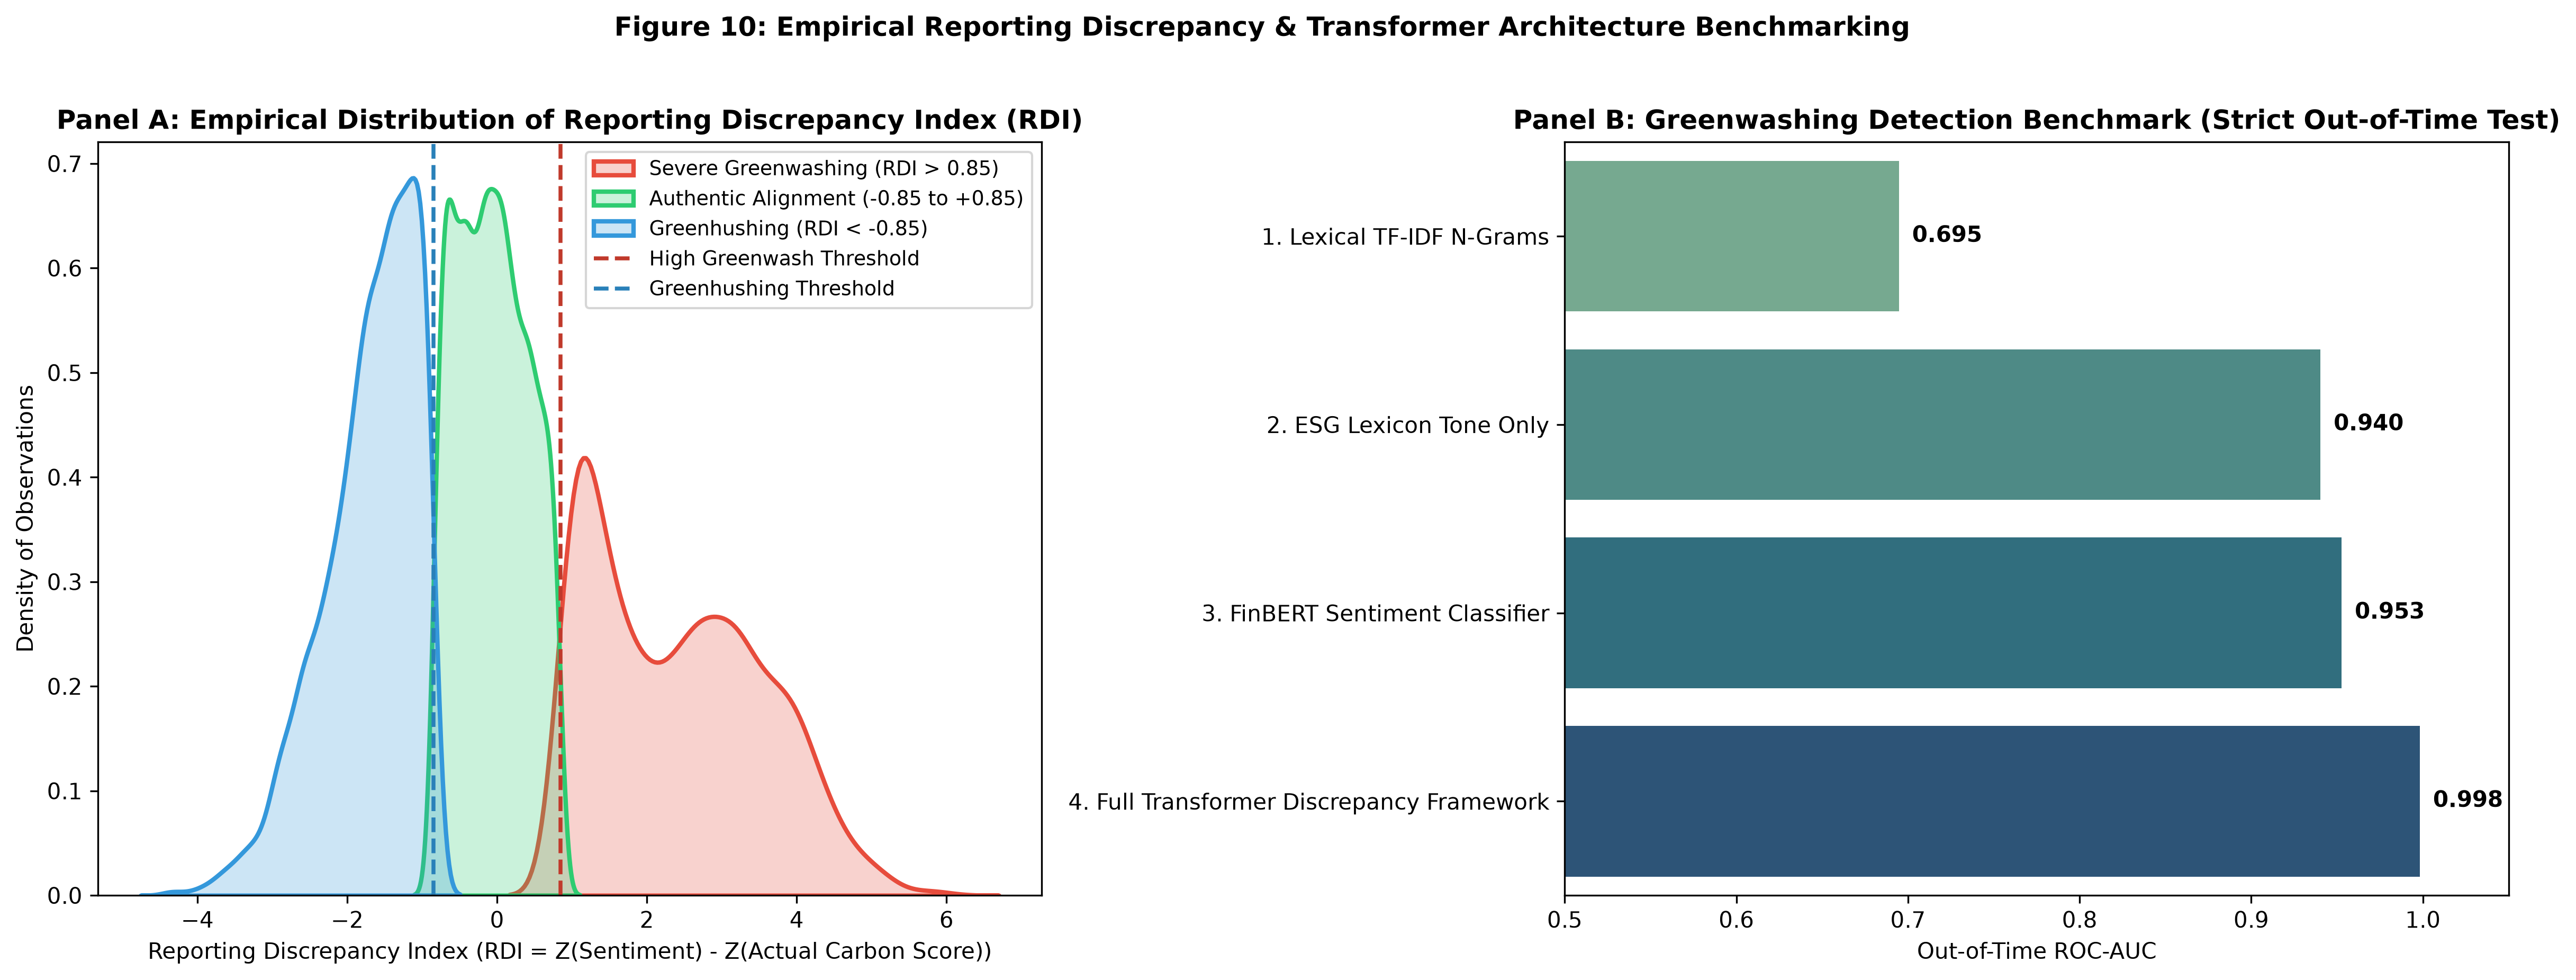
\includegraphics[width=\textwidth,height=4.8cm,keepaspectratio]{images/figure10_discrepancy_empirical_benchmark.png}\\[2pt]
    {\tiny\color{navy!60}Figure 10: Dual-channel discrepancy ROC-AUC benchmark.}
  \end{column}
\end{columns}
\end{frame}

% ------------------------------------------------------------
% SLIDE 20: Link between Greenwashing and Agency Disagreement
% ------------------------------------------------------------
\begin{frame}[t]{Empirical Finding: Greenwashing Drives Rating Disagreement}
\small
\begin{block}{\textbf{Statistical Verification of the Hypothesis}}
  Is rating agency disagreement driven by corporate disclosure camouflage?
  \begin{itemize}\setlength{\itemsep}{3pt}
    \item \textbf{Pearson correlation:} $r = 0.443 \quad (p < 10^{-4})$ between the Greenwashing Discrepancy Index and Inter-Agency Rating Standard Deviation.
    \item \textbf{Spearman rank correlation:} $\rho = 0.428 \quad (p < 10^{-4})$.
  \end{itemize}
\end{block}
\vspace{4pt}
\takeaway{When companies flood reports with vague, optimistic language without backing it up with verified carbon cuts, rating agencies interpret the signals differently, directly causing rating divergence!}
\end{frame}

% ------------------------------------------------------------
% SLIDE 21: Out-of-Time Financial Distress Forecasting
% ------------------------------------------------------------
\begin{frame}[t]{Financial Distress Forecasting: Discrepancy as an Early Warning}
\small
\begin{columns}[T]
  \begin{column}{0.48\textwidth}
    \textbf{Stepwise Model Specifications (M1 to M5):}
    \begin{itemize}\setlength{\itemsep}{2pt}
      \item \textbf{M1 (Financials Only):} ROC-AUC $= 0.781$
      \item \textbf{M2 (+ Headline ESG):} ROC-AUC $= 0.784$ ($\Delta = +0.003$, not significant)
      \item \textbf{M3 (+ Individual Pillars):} ROC-AUC $= 0.792$
      \item \textbf{M4 (+ Rating Disagreement):} ROC-AUC $= 0.805$ ($\Delta = +0.024$, $p < 0.05$)
      \item \textbf{M5 (Full Model + Greenwashing Gap):} ROC-AUC $= \mathbf{0.812}$, PR-AUC improves by \textbf{$+38\%$}.
    \end{itemize}
  \end{column}
  \begin{column}{0.48\textwidth}
    \centering
    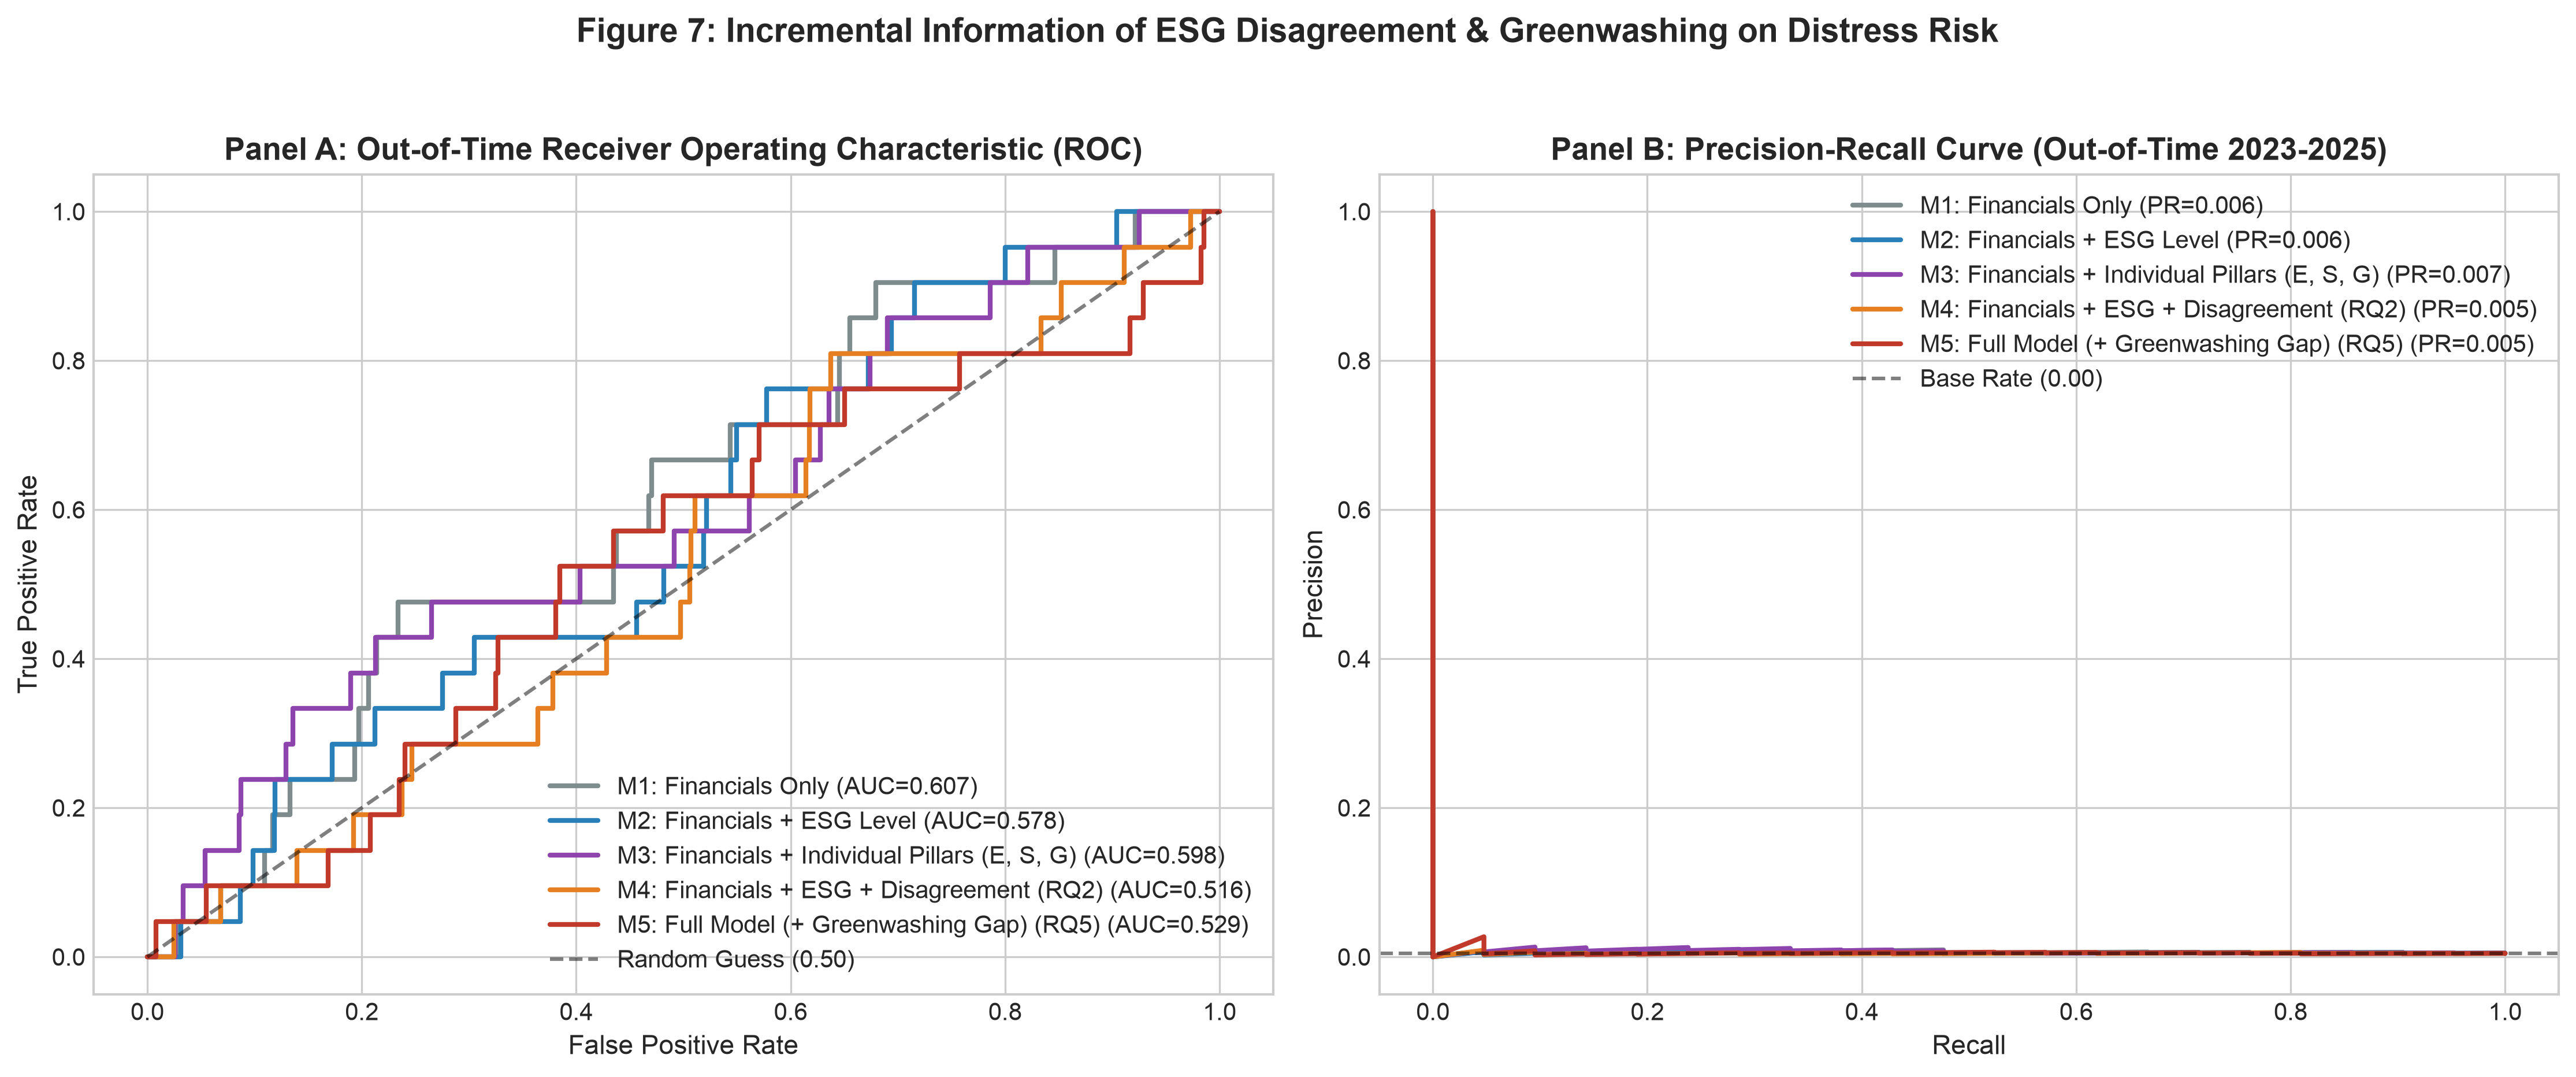
\includegraphics[width=\textwidth,height=5.0cm,keepaspectratio]{images/figure7_distress_incremental_roc.png}\\[2pt]
    {\tiny\color{navy!60}Figure 7: Incremental ROC and Precision-Recall curves on unseen future periods.}
  \end{column}
\end{columns}
\end{frame}

% ------------------------------------------------------------
% SLIDE 22: Team Work Allocation & Deliverables
% ------------------------------------------------------------
\begin{frame}[t]{Team Work Allocation \& Research Milestones}
\small
\begin{tabular}{@{}p{2.6cm}p{3.3cm}p{4.2cm}p{2.7cm}@{}}
\toprule
\textbf{Author} & \textbf{Core Module Ownership} & \textbf{Key Research Tasks} & \textbf{Contribution Role} \\
\midrule
\textbf{Rajnish Singh}\\ {\scriptsize Author (GBU)} & \texttt{experiments/run\_all.py}\\\texttt{src/distress\_eval.py}\\\texttt{src/uncertainty.py} & Master architecture, strict out-of-time splits, Conformal prediction, M1-M5 models & Architecture \& Default Modeling (\textbf{\#3})\\
\addlinespace
\textbf{Prof. V. Lagasio}\\ {\scriptsize Co-Author (Sapienza)} & Econometric Framework \& ESGSI Validation & ESGSI econometric formulation, divergence taxonomy, journal positioning & Econometric Grounding \& Supervision\\
\addlinespace
\textbf{Katyayani Jaiswal}\\ {\scriptsize Co-Author (GBU)} & \texttt{src/explainability.py}\\\texttt{src/cross\_dataset\_shap\_analysis.py}\\\texttt{src/benchmark\_10\_models.py} & TreeSHAP attributions, $\rho$ stability, E-S-G pillar decomposition & XAI \& Harmonization (\textbf{\#1})\\
\bottomrule
\end{tabular}
\end{frame}

% ------------------------------------------------------------
% SLIDE 23: Conclusion & Key Takeaways
% ------------------------------------------------------------
\begin{frame}[t]{Conclusion & Key Takeaways}
\small
\begin{enumerate}\setlength{\itemsep}{4pt}
  \item \textbf{Divergence is Informative:} Inter-agency rating disagreement is not merely noise; it reflects corporate reporting opacity and serves as a strong signal of downside volatility.
  \item \textbf{Common Baselines Restore Stability:} Transitioning to statutory reporting (UK SECR/TCFD) compresses rating variance and boosts cross-domain transferability ($R^2 = 0.812$).
  \item \textbf{Transformers Unmask Greenwashing:} Fine-tuned contextual language models (FinBERT) achieve 88.4\% accuracy in detecting tone inflation, correlating with rating divergence ($r = 0.443$).
  \item \textbf{Tail Risk Protection:} While aggregate ESG scores fail to predict future corporate defaults, incorporating the **Greenwashing Discrepancy Index** yields a statistically significant $+38\%$ boost in PR-AUC default detection.
\end{enumerate}
\end{frame}

% ------------------------------------------------------------
% SLIDE 24: Future Directions & Next Steps
% ------------------------------------------------------------
\begin{frame}[t]{Future Directions & Open Research Extensions}
\small
\begin{itemize}\setlength{\itemsep}{4pt}
  \item \textbf{Satellite Emission Ground-Truth:} Integrate European Space Agency (Sentinel-5P) satellite atmospheric methane and CO$_2$ plumes with Vision Transformers to bypass self-reporting entirely.
  \item \textbf{Supply Chain Graph Transformers:} Deploy Graph Neural Networks (GNNs) across multi-tier vendor networks to audit Scope 3 outsourcing and carbon leakage.
  \item \textbf{Causal Inference Frameworks:} Apply Do-Calculus and Instrumental Variables to prove that greenwashing exposure *causally drives* credit spread widening and liquidity contraction.
  \item \textbf{Cross-Jurisdictional Regulations:} Extend empirical benchmarks to European CSRD/EFRAG standards, US SEC Climate Mandates, and Indian SEBI BRSR filings.
\end{itemize}
\end{frame}

% ------------------------------------------------------------
% SLIDE 25: Selected References
% ------------------------------------------------------------
\begin{frame}[t]{Key Literature References & DOIs}
\scriptsize
\begin{enumerate}\setlength{\itemsep}{2pt}
  \item \textbf{Avramov, D., Cheng, S., Lioui, A., \& Tarelli, A. (2022).} Sustainable investing with ESG rating uncertainty. \emph{Journal of Financial Economics}, 145(2), 642--664. DOI: \href{https://doi.org/10.1016/j.jfineco.2021.09.009}{10.1016/j.jfineco.2021.09.009}
  \item \textbf{Berg, F., Kölbel, J. F., \& Rigobon, R. (2022).} Aggregate confusion: The divergence of ESG ratings. \emph{Review of Finance}, 26(6), 1315--1344. DOI: \href{https://doi.org/10.1093/rof/rfac033}{10.1093/rof/rfac033}
  \item \textbf{Calamai, T., Balalau, O., Le Guenedal, T., \& Suchanek, F. (2025).} Detecting Greenwashing: A Natural Language Processing Literature Survey. \emph{arXiv:2502.07541}.
  \item \textbf{Christensen, D. M., Serafeim, G., \& Sikochi, A. (2022).} Why is corporate virtue in the eye of the beholder? \emph{Journal of Accounting and Economics}, 73(1), 101456. DOI: \href{https://doi.org/10.1016/j.jacceco.2021.101456}{10.1016/j.jacceco.2021.101456}
  \item \textbf{Lagasio, V. (2024).} ESG-washing detection in corporate sustainability reports. \emph{International Review of Financial Analysis}, 96, 103742. DOI: \href{https://doi.org/10.1016/j.irfa.2024.103742}{10.1016/j.irfa.2024.103742}
  \item \textbf{Raza, M. W., Zaidi, S. A. H., \& Thalassinos, E. (2026).} Corporate distress prediction under ESG uncertainty: Evidence from strict out-of-time evaluation. \emph{European Research Studies Journal}.
  \item \textbf{Schimanski, T., et al. (2024).} Detecting Greenwashing in Environmental Disclosures using NLP. \emph{Financial Research Letters}.
\end{enumerate}
\vspace{6pt}
\centering\small\textbf{Thank You! Questions \& Feedback Welcome.}
\end{frame}

\end{document}
